\documentclass[LaM,noexaminfo,oneside,binding=0.6cm]{sapthesis}

\usepackage{float}
\usepackage{tikz}
\usepackage{varwidth}
\usepackage{geometry}
\usepackage{marginnote}
\usepackage{url}
\usepackage{hyperref}
\usepackage{placeins}
\usepackage{xcolor}
\usepackage{svg}
\usepackage{changepage}
\usepackage{colortbl}
\usepackage{tabularx}
\usepackage{multirow}
\usepackage{enumitem}
\usepackage{comment}

\graphicspath{ {pics/} }

\definecolor{dummy-cyan}{HTML}{0099cd}
\definecolor{dummy-yellow}{HTML}{fcc013}
\definecolor{dummy-orange}{HTML}{f2a147}
\definecolor{dummy-green}{HTML}{00afaa}
\definecolor{dummy-red}{HTML}{e73e51}
\definecolor{dummy-red-strong}{HTML}{3D0814}
\setlength\arrayrulewidth{1.5pt}
\arrayrulecolor{dummy-yellow}



%Definition

\newcommand{\definition}[3][\textwidth-\pgfkeysvalueof{/pgf/inner xsep}-2mm]{

\begin{figure}[H]
    \reversemarginpar
    \marginnote{\includesvg[width=2cm]{def-icon.svg}}
    \begin{tikzpicture}
    
    
    \node[line width=.5mm, draw=dummy-yellow,  text width=#1, anchor=north west] (text) {\vspace*{25pt}\\\begin{adjustwidth}{10pt}{10pt}#3 \medskip \end{adjustwidth}};
    
    \node[text=white,anchor=north west,align=center, minimum height=25pt] (label) at (text.north west) {\LARGE#2 \hspace*{.5mm}};
    
    \path[draw=dummy-yellow,line width=.5mm,fill=dummy-cyan] 
        (text.north west) --
        (text.north east)  --
        (text.north east|-label.south east) --
        (text.north west|-label.south west) -- cycle;
        
    \node[text=white,anchor=west,align=center, minimum height=20pt] (label_2) at (label.west) {\LARGE \textbf{DUMMY} definition for \textbf{#2}\hspace*{.5mm}};

    \end{tikzpicture}
\end{figure}
\FloatBarrier
\noindent
}

\renewcommand\tabularxcolumn[1]{m{#1}}

\endinput


\hypersetup{
    colorlinks,
    citecolor=black,
    filecolor=black,
    linkcolor=black,
    urlcolor=black
}



\courseorganizer{Sapienza University of Rome}
\advisor{Silvia Bonomi}
\course[override]{Master's Degree in Engineering in Computer Science}
\IDnumber{1649359}
\submitdate{2020/2021}
\copyyear{2022}
\authoremail{edo.puglisi95@gmail.com}
\author{Edoardo Puglisi}
\title{Cyber Risk Management for Dummies}
\subtitle{The Hitchhiker's Guide to Critical Infrastructures}





\begin{document}

\frontmatter
\maketitle
\dedication{} 


\mainmatter



\tableofcontents

\chapter*{Introduction}
\addcontentsline{toc}{chapter}{Introduction}
In the last few years, Cyber Risks Management became a core practice inside any organization which deal with full or partially digital assets (intended as all those resources that depend in some way on a computer). Or so it should be. The presence of smart devices and ever-increasing connectivity have led organizations to work within cyberspace with its benefits and dangers. Not everyone is ready for this journey and some will succumb along the way. And this is where I come into play. My task is to provide you with a guide that can benefit everyone, regardless of their skill level, from beginners to experts, from dummies to masters, and which lays the foundations for the research towards the much desired cybersecurity. The answer to all your questions will not be "42", but something a little bit more complicated. This work is presented as a guide and is structured as such, but don't expect instructions like those of "Ikea" fornitures. Numerous approaches to cyber risk management will be shown and analyzed. What steps must be followed for a correct use of cyberspace? We will have at our disposal systematic methodologies to detect and reduce vulnerabilities and threats (e.g. MEHARI, OWASP etc.) or more complex and structured frameworks such as the Cyber Security Framework provided by NIST. There will be dummy-proof examples (I tried very hard to get to that level) and colorful figures. The final focus of this survey will be cyber risk management within critical infrastructures, in particular healthcare infrastructure. In the last period, in fact, healthcare has been the victim of numerous cyber attacks and my goal is to explain why and how to prevent this from happening again.\newline
The rest of the survey is organized as follows. Chapter 1 introduces the concept of risk management within an organization (but outside the cyberspace) by examining ISO-31000 risk management framework. Chapter 2 shifts the focus to the cyber component of risk management, briefly listing the new opportunities and problems that cyberspace offers us. Taking into consideration the benefits and dangers of cyberspace, chapter 3 analyzes the main "weapons" available to those we will call guardians of the cyberspace, chapter 4 lists the main methodologies to face systematic cyber threats and chapter 5 details some of the major cyber risk management frameworks and their similarities and differences. These three chapters are strongly connected to each other: CRM methodologies make use of different tools and frameworks can adapt them to fit the organization's mission. Chapter 6 evaluates the current situation in healthcare infrastructure in the field of cybersecurity, proposes some solutions to the problems highlighted and a "dummy" example of what is the process to implement cyber risk management controls inside a hospital. Chapter 7 draws the conclusions. Let the journey begin.

\chapter{Risk Management}
The main purpose of this guide is to discuss how modern enterprises should manage cyber-risks while interacting inside critical environments. But before entering in details of all of this we have to understand what is risk management in general. "What is a risk ?", "Why does everyone talk about risk management ?", "I am a farmer: is it really important for my cucumber farm ?", "How do I implement it inside my organization ?". These and other questions will be answered in details in the following sections.
\section{What is it?}
History of risk management originates in the Tigris-Euphrates valley about 3200 B.C. (exactly like everything we studied at school). There lived a group called the Asipu and one of their main function was to serve as consultant for uncertain or difficult decisions: they would identify the important dimensions of the problem, the alternatives and collect data on the outcomes of each of them. After the analysis was completed, they would recommend the most favorable alternative issuing a final report to the client in a not at all uncomfortable clay tablet. The bad part is that the best available data were divine signs, not easily quantifiable, and if the prediction was faulty they could easily blame a playful God. Fortunately things changed a bit through the years and human started using more easy to read signs such as probability, even though the old techniques for mitigating or reducing risks are still very effective and used \cite{Covello1985}.
Back to the present, every business or enterprise, from the small corner store to the large manufacturer, faces risks everyday: factory buildings can be damaged by fire slowing the supply chain, an employee could slip, fall and then sue the manager costing money to the company, financial losses can occur as a result of defective products or data breaches can damage the reputation of a data controller after the violation of the privacy of its users.
All of these are simple examples of risk, which may span across every kind of sector (not only cyber-related).
\definition{Risk}{\begin{center}"Effect of uncertainty on objectives" \cite{ISO2018}\medskip\end{center}  Practically speaking, a risk is "the possibility of something bad happening", in every possible context an organization may operate. A risk can be objective or quantifiable such as a financial loss or subjective and difficult to quantify such as a reputation loss.}Risk management, as you may understand by yourself, aims to manage every risk situations inside an organization. More technically is a continuous, gradual and proactive process that aim to "direct and control the organization with regard to risk" \cite{ISO2018}: in few words, reduce the likelihood of risks to prevent disasters. Fundamental purpose of enterprise risk management, anyway, is not to just protect, but enhance and create value for the organization. An organization recognized as safe will certainly be preferred to one with serious security flaws and therefore will have greater opportunities for investment or contractual proposals.
\section{Is it important?}
Of course it is, otherwise we wouldn't be here talking about it. The goal of every successful business is to gain value and reduce losses (both in terms of money, reputation and so on) and risk management is the dividing line between these two scenarios. Focusing the attention on risk, a business can (try to) protect its assets (those things on which protection is worth investing) before it's too late. The saying "prevention is better than cure" also applies in this context: investing in prevention certainly has a cost, but in most cases it is lower than the cost of treatment in case of disaster (and reduces the likelihood of such disaster). When a potential risk has been identified, mitigate it is (most of the times) easy or at least doable. Managing the after effects of a risk, instead, is harder and not always possible: is it easier and more convenient to prevent a fire putting in place a working fire extinguishing system or to rebuild the entire burned-out building?\newline
Going back to the farmer question: YES! Also a cucumber plantation has risks (flooding, heating, parasites and other environmental risks) and a good farmer has to manage them in a proper way, for example using pesticides to prevent parasites that would destroy the plantation (other cucumber risks are not covered in this paper).
We can use the farmer as an example to introduce other important element of risk management, the stakeholder.
\definition{Stakeholder}{\begin{center}"Person or organization that can affect, be affected by, or perceive themselves to be affected by a decision or activity." \cite{ISO2018}\medskip\end{center} Simply the ones that will pay the consequences of anything that was decided regarding risk: if a flood destroy the culture, the farmer won't be able to sell cucumbers at Sunday market, losing money and clients. The farmer is the stakeholder: his decision to not invest in "anti-flood" measures led him to no longer have anything to sell.}
\section{How to implement it?}
The term Risk management refers to the set of processes through which an organization identifies, analyzes, quantifies, eliminates and monitors the risks associated with a specific production process. We stated before that risk management is a continuous, gradual and proactive process that aim to reduce risks or at least the damage caused by them. Gradual because is subdivided in multiple subsequent steps with different features and goals. Proactive because focuses mainly on prevention from incidents, reducing risks' likelihood, and not on the recovery from the derived problems (that is anyway a crucial part of every business: every organization should have a B plan). Continuous because is repeated in loop, adding at each iteration additional information acquired from previous one and improving itself. But! Here rises a problem. The process we are talking about is not properly step-by-step and there isn't a guide to follow with the exact actions to take inside each organization. Different organizations have to satisfy different requirements (also imposed by government) according to own area of expertise, size or geographic location, and it is not feasible to write a different process for each of them. For this reason someone decided to write down the guidelines and best practices that should (NOT must) be followed for an healthy risk management plan. Some of the brightest minds on earth grouped together to draw up what are called \textit{standard}.\definition{Standard}{\begin{center}A published statement on a topic specifying characteristics, usually measurable, that must be satisfied or achieved in order to comply with the standard." \cite{Paulsen2019}\medskip\end{center} Risk management standards are like a guide to help ensuring that risk management is carried out in a proper way. Standards usually include checkpoints and examples, to make it really easy for organizations to comply with them (exactly like this guide, maybe it will be converted in standard in the near future).}"ISO 31000" by \textit{International Organization for Standardization} (ISO) and "Enterprise Risk Management" by \textit{The Committee of Sponsoring Organizations of the Treadway Commission} (COSO) are the two leading risk management standards in the world today. Even though they are very similar (trivially they have the same goal) differences between them far outnumber similarities. COSO ERM is targeted more toward people in accounting and audit while ISO 31000 is written for anyone interested in risk management. ISO 31000 is few pages long while COSO ERM needs you to take holidays to finish it. The choice between one or the other consists on which one fits the organization and the good part of this game is that is possible to choose all of them (or others) and take the best of each. In the following section we will see an overview of ISO 31000 to get an idea of how these standards are structured, but going on with this guide we will focus on more specific standards for cyber-related risk and their methodologies.

\section{Standard example: ISO 31000}
I decided to use ISO 31000 \cite{ISO2018} as example, for few basic reasons: is concise, easy to follow, can be read in less than an hour and can be applied to pretty much any industry, culture, and language. The standard consists of 3 main components: Principles, Framework and Process. Let's deepen it together. 
\subsection{Principles}
The principles are the characteristics that an effective and efficient risk management should have, communicating its value and explaining its intention and purpose. The principles are the core element for managing risk and should be considered when establishing the organization’s risk management framework and processes. These principles should enable an organization to manage the effects of uncertainty on its objectives. Consider them the "eight" commandments.
\begin{figure}[H]
  \centering
  \includesvg[inkscapelatex=false,width=0.5\textwidth]{iso-1.svg}
  \caption{Principles}
\end{figure}
\noindent
\begin{itemize}
    \item \textbf{Integrated:} Risk management is a fundamental part of all activities inside an organization.
    \item \textbf{Structured and comprehensive:} The approach to risk management should be structured and comprehensive in order to have consistent and comparable results. It's not a free-for-all!
    \item \textbf{Customized:} Risk management framework and process can be customized by each organization to fit their own context and objectives. 
    \item \textbf{Inclusive:} Is important to involve stakeholders in risk management plan and consider their knowledge, view and perceptions while making decisions. This results in improved awareness and informed risk management.
    \item \textbf{Dynamic:} Organization's internal and external context can change rapidly and risk can emerge, change or disappear just as quickly. Risk management must anticipates, detects, acknowledges and responds to those changes as soon as possible.
    \item \textbf{Best available information:} Historical and current information, as well as future expectations are the inputs of risk management. Risk management takes into account any limitations and uncertainties associated with such information and expectations. Information should be timely, clear and available to relevant stakeholders.
    \item \textbf{Human and cultural factors:} Risk management is significantly influenced by human behaviour and culture at each level and stage.
    \item \textbf{Continual improvement:} Risk management is a loop that improve itself at each iteration.
\end{itemize}
\subsection{Framework}
A Risk management framework assists organization in integrating risk management into its main activities and functions. Its effectiveness will depend on its degree of integration into the governance of the organization, that is the system by which an organization makes and implements decisions in pursuit of its objectives. The more or less pyramidal system in which the boss at the top gives orders to the subordinates of the lower levels, but for which he has the responsibility and on which the fate of the organization depends. Fundamental is the support from stakeholders, in particular from top management. Its features, modeled around Leadership and Commitment, are subdivided into Integration, Design, Implementation, Evaluation and Improvement, taking into account the fact that the way in which they work together should be customized to the needs of organization.
\begin{figure}[H]
  \centering
  \includesvg[inkscapelatex=false,width=0.5\textwidth]{iso-2.svg}
  \caption{Framework}
\end{figure}
\noindent
\subsubsection{Leadership and commitment}
In risk management framework, everything rotates around top management and oversight bodies. They should ensure (if they don't want to be fired) that risk management is well integrated into all organizational activities, demonstrating leadership and commitment. They are required to: customize and implement inside the organization all components of the framework, issue a set of rule or guidelines for the desired risk management approach, ensure the availability of necessary resources, subdivide the authority, responsibility and accountability at appropriate levels within the organization.
All of this will help the organization to align risk management with its objectives and strategy, recognize and address all obligations and voluntary commitments, establish which kind of risk (and how many) the organization should take, inform the stakeholders about them and the importance of their management, promote monitoring and ensure that the framework remains coherent with the context of the organization.\newline
Oversight bodies answer the question "Who controls the controller?" If the top management is required to manage risk, the oversight bodies are accountable for overseeing risk management. Their main tasks are: ensure that risks are taken into account during organization's objectives setting, understand the possible risk that may rise while facing these objectives, ensure that the managing system is well implemented and operative and that every important information about risk and their management is communicated in the proper way.
\subsubsection{Integration}
"To conquer fear, you must become fear" said Ra's al Ghul to Bruce Wayne in the process of transformation into Batman. Same story to integrate risk management into organizational structure. I'm not asking you to become the structure of your organization anyway, just to understand it. Structures differ depending on the organization's purpose, goals and complexity and risks may rise in every part of them, giving a portion of responsibility for managing risk to everyone. Risk management should be part of the behaviour of the organization (purpose, governance, strategy and objectives) and not a separated entity.
\subsubsection{Design}
First things first, understand the organization and its context, both internal (e.g. vision, mission and values of organization) and external (e.g. geographic area and external relationships).\newline
Top management and oversight bodies should demonstrate and articulate their commitment to risk management through a policy or whatever form of document that clearly expresses organization's objectives and commitment to risk management. This should be communicated within organization and to stakeholders.\newline
A correct risk management framework design requires a proper subdivision of roles (authorities, responsibilities and accountabilities) and allocation of appropriate resources (people, skills, documents, training).\newline
Last but not least: communication and consultation. Communication means sharing information with targeted audiences. Consultation means listening to feedback to shape decisions or other activities.
\subsubsection{Implementation}
Previous steps are important, but now is time to make them effective. Organization should develop an appropriate plan including time and resources, identify where, when, how and by whom decisions are made modifying the decision-making processes if needed and ensure that all necessary arrangements are well understood and practised. Like always, stakeholders should be engaged and aware to take into account any new or subsequent uncertainty as it arises.\newline
Design and Implementation will ensure that risk management is part of all activities within the organization.
\subsubsection{Evaluation}
The organization should periodically measure the framework performance against expected results and determine whether it is still efficient to support achieving the objectives.
\subsubsection{Improvement}
Follows the "Improvise. Adapt. Overcome" Bear Grylls's mentality, without the part of improvisation. Organization should monitor internal and external changes to adapt the risk management framework to them. Continually improving the suitability, adequacy and effectiveness of the risk management framework contributes to the enhancement of risk management.
\subsection{Process}
As said before, the risk management process is an iterative loop that like previous elements should be integrated in into the structure, operations and processes of the organization. Inside an organization there can be many applications of risk management process, customized to achieve the objectives.
\begin{figure}[H]
  \centering
  \includesvg[inkscapelatex=false,width=0.5\textwidth]{iso-3.svg}
  \caption{Process}
\end{figure}
\noindent
\subsubsection{Communication and consultation}
Stakeholders have to understand risk, know the basis on which decisions are made and why particular actions are required. The purpose of Communication and consultation is just that: the first aims to promote awareness providing, for example, sufficient information to facilitate risk oversight and decision-making, the latter involves obtaining feedback and supporting decision-making ensuring that different views are appropriately considered during the process. Both internal and external stakeholders should be part of the communication and consultation step.
\subsubsection{Scope, context and criteria}
To adapt the process to the organization's profile is necessary to establish the scope, the context and criteria.\newline
The scope regards the organizational objectives that must be taken into account at all different levels of the risk management process (e.g. strategic, operational, programme, project, or other activities). Is important to consider objectives and decisions that need to be made, the expected outcomes from each step, required resources, tools and techniques and relationship with other projects or activities.\newline
Context, internal or external, is the environment in which the organization seeks to define and achieve its objectives and where the risk management process is applied. Understanding the context is fundamental because, trivially, is where the risk may rise (at least the one the organization is interested in).\newline
Criteria are used to evaluate the type of risk that organization may or may not take, their significance and to support decision-making process. They should reflect the organization's values, objectives and resources: chip shortage is a risk that our farmer friend can take without problems. Criteria should be established at the beginning of the risk management process, but being dynamic they should be continually reviewed.
\subsubsection{Risk assessment}
Risk assessment consists of risk identification, analysis and evaluation. It should be conducted systematically, iteratively and collaboratively and should use the best available information, supplemented by further enquiry as necessary.\newline
Identification means find, recognize and describe the risks that may disturb organization's path to the success. The goal is to identify uncertainties (whether or not their sources are under organization's control) that may effect one or more objectives.\newline
Risk analysis aims to understand the nature of risk and its level. Given the fact that we are talking about uncertainty, the more information about risk are available the easier will be to comprehend it: sources, consequences, likelihood, events, scenarios, controls and their effectiveness. The analysis complexity may change according to its purpose or availability of information, can be qualitative, quantitative or a combination of these depending on circumstances.\newline
Risk evaluation supports decisions: compares results of risk analysis with risk criteria to determine where additional action is required (e.g. reconsider objectives or further analysis).
\subsubsection{Risk treatment}
Self explanatory: how should we handle the risk? An iterative (again) process that consists of: formulating and selecting risk treatment options, planning and implementing them, assessing their effectiveness, deciding whether the remaining risk is acceptable or not (in this case more treatment needed).\newline
To select the best treatment option(s) is necessary to balance potential benefits with costs, effort and disadvantages of implementation. Common options are risk sharing (e.g. buying insurance), change likelihood or consequences, remove sources, take more risk or completely avoid the activity that generate the risk. Note that the criteria used to choose the right option is not solely economic, but take into account all organization's obligations: it would be a lot easier, for the farmer, to spread an huge amount of insecticide to protect his cultivation, but this may violate the limits imposed by law.\newline
When the best option is chosen, is time to prepare and implement the risk treatment plan: what is the implementation order of the treatment? Who is accountable and responsible for implementation? Which resources are required? What are the actions to be taken? When?
\subsubsection{Monitoring and review}
An iterative process wouldn't have made sense without its constant monitoring. Ongoing monitoring and periodic review assure and improve the quality and effectiveness of process design and should take place in all stages of it, with clearly defined responsibilities.
\subsubsection{Recording and reporting}
All information resulting from the risk management process should be recorded and reported through appropriate mechanisms. Reporting is fundamental in the organization’s governance and should enhance the quality of dialogue with stakeholders and support top management and oversight bodies in meeting their responsibilities.\vspace{3cm}\newline
This wall of text may have been difficult to digest. And that's just the beginning! But let's try to make sense of it. The framework examined is only one of the many used by organizations, some features may (and will) differ from those of other standards and no one will ever ask you to follow every step of any framework you want to implement to the letter. The framework acts as a backbone, as a model to follow, but it is not a checklist to complete. The "suggested" actions (you must however follow them wisely) have the aim of increasing the synergy between the technologies in use, the processes in which they are used and the people who use them. It is important to grasp all the relationships between the components (human or not) within the organization and the framework provides guidelines to do this in the best possible way.


\chapter{Cyber Risk Management}
At this point you should have a good overview of what risk management is. As you can see it is not like a magic formula that solves all problems just saying it, but it must be interpreted and adapted according to the situation. It is however a good starting point! 
Anyway, like technology, risk management has evolved over the years: there are new types of entities to protect from so many new types of risk and as many new ways to deal with them. If you enjoyed risk management, get ready for CYBER risk management!
\section{Why cyber?}
<<wHaT DoEs "CyBeR" mEaN?>> you may ask. Simply the abbreviation for \textit{cyberspace}.
\definition{Cyberspace}{\begin{center}"A global domain within the information environment consisting of 
the interdependent network of information systems infrastructures including the Internet, telecommunications networks, computer systems, and embedded processors and controllers." \cite{Paulsen2019}\medskip\end{center} Long story short: the "place" where communications between digital devices occur (the "Matrix" if you need a pop culture example).}Cyberspace is a (mostly) virtual environment composed by sensors, signals, connections, transmissions, processors and controllers inside which streams of data flow. It can be small like your private network at home or huge like the whole Internet, it can be virtual-only or include physical elements (cyber-physical systems). This universe of digital networks and computers is a new cultural and economic front, a world in which multinationals, corporations and computer pirates clash for the conquest of data and information. The so-called Fifth Domain, after Air, Earth, Sea and Space. Cyberspace nowadays is "visited" by everyone and is fundamental for every kind of business: when you check your emails or bank account you (your information) are navigating the cyberspace, when you order an hawaiian pizza you are navigating the cyberspace too (the fact that you should be arrested for this is an other story though). Billions of people everyday enter the cyberspace for any kind of reason and this gives a large number of possibilities to  malicious actors: both the victim and the author of these attacks space from common citizen to governments. Cyberspace will be the battlefield in which we will spend most of this journey and that's why it is called cyber risk management: fasten your seat belt!
\section{Modern problems...}
We moved from risk management to cyber risk management. Fine. Why?\newline
Basically because what is now important for us, what requires our attention on current days, is in an intangible form and populates cyberspace. Our whole life is almost fully dependant from digital resources: no more queues at bank for financial operations thanks to bank accounts accessible from computers or smartphones, our data are accessible worldwide via cloud storage at high speed and you can play \textit{Fortnite} all day long online with your friends. What a time to be alive! But how risks inside an intangible world such as cyberspace can hurt our real world?\newline
It's April 2011. You just got back from school and turn on your \textit{Playstation 3}, ready to play an online team deathmatch with your friends on \textit{Call Of Duty: Modern Warfare 2}. What's wrong? You notice that you can't connect to \textit{Playstation Network} even though you payed the subscription with all your pocket money. You start crying.\newline
\cite{Sheppard2013} highlight that what might have seemed to you like a trivial connection problem, was actually an huge cyber attack towards \textit{Sony's Playstation Network} by an organized group of hackers and what for you was a little unexpected afternoon for Sony was a big financial loss. Interruption of online services caused a loss of \$170 million for repair costs and 77 million credit card numbers were stolen. Taking into account losses from stolen information and legal actions the final figure may be far higher at \$1-2 billion. Sony's slow response to acknowledge the attacks and lack of transparency contributed to the loss and the reputational damage that also led to stock losses. Unlike natural disasters, whose consequences can be easily understood and contained, cyber attacks have unique risk characteristics and can be insidious and systemic. The potential costs of an attack or series of attacks is not limited to a geographical area or a company’s reputation, but can ruin entire industries as well as upset the stability of a nation.\newline
The assault on the diligence of yesterday, today is represented by the cyber criminals who attack our communications, the outlaw who used to rob the saloon is now a hacker who tries to steal your bitcoin wallet. The bad guys have always been and always will be, the problem is that they now have many more ways to attack. It is also necessary to specify that many critical infrastructures are almost totally dependent on informatic systems and, as explained in \cite{Solms2013}, it is important to make a distinction between information security and cyber security: not only information is in danger, but also private and public safety. The mere fact that your personal data is stolen may not matter, but it is their inappropriate use such as identity theft that should worry you.
\subsection{Threats}
The term \textit{threat} will be used a lot since identify the evil that we must defeat for the rest of this paper, in particular a cyber-threat is a threat that exploits a cyberspace.
\definition{Threat}{\begin{center}"Any circumstance or event with the potential to adversely impact organizational operations (including mission, functions, image,or reputation), organizational assets, individuals, other organizations, or the Nation through an information system via unauthorized access, destruction, disclosure, modification of information, and/or denial of service." \cite{Paulsen2019}\medskip\end{center} No explanation required I hope.}Threats are generally divided in \textit{malicious} and \textit{nonmalicious} on the basis of their source: malicious threats are caused by intentional attacks that aim to harm the organization in any possible way (e.g. organized group of hackers brute forcing organization's database), while nonmalicious ones are caused by incidents, unintentional events that can be caused also by internal staff (e.g. crash due to programming errors). There exists anyway multiple classification methods for threats. The most common ones are based on attacks techniques used by adversaries to put the attack in place or based on the impact that the threat will produce on the organization if succeed, but the methods can be mixed and adapted to create totally new ways of classification as exposed in \cite{Jouini2014}. Here are some of the most common examples of threats that an organization may face.

\subsubsection{Denial of Service}
Good old \textit{DoS} attack, maybe the most common and well-known type of threat among the general public. It consists of a cyber attack that floods a computer or network so it can’t respond the requests that instead are important. The DoS attack can also be performed from a computer network instead of a single computer: in this case we talk about Distributed Denial of Service (DDoS). A particular example of DDoS is the \textit{Botnet}: exploiting malwares (more later) millions of systems can be infected and controlled by a hacker that aims them towards a single target overwhelming its processing capabilities. Being spread in different geographic locations botnets are (usually) hard to trace. The example I gave you before, the attack towards Playstation Network, was exactly a denial of service that generated an huge loss to Sony.

\subsubsection{Malware}
Malware is what your mother would call "virus" and she wouldn't be completely wrong. Malwares are malicious software (spyware, ransomware, virus and worms) that are inserted coverly into a system with the intent of compromising the confidentiality, integrity or availability of victim's data, applications or operating system. In May 2017, years before Covid-19, an other (cyber) epidemic broke out due to the ransomware called \textit{WannaCry}: when infected, the victim's system was encrypted and the user was forced to pay a \textit{ransom} in Bitcoin for decryption (this gives the name to ransomware). Imagine of turning on your laptop and seeing the picture below: you would cry for sure.
\begin{figure}[H]
  \centering
    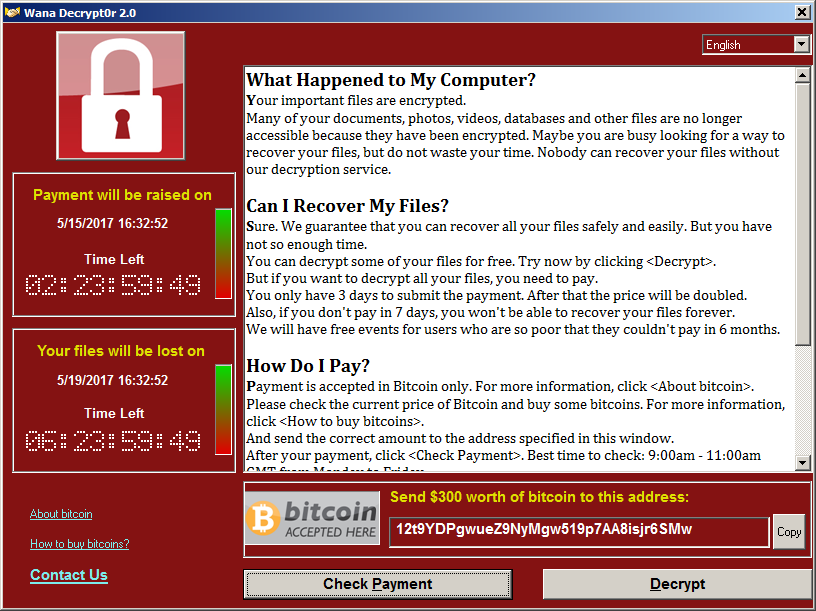
\includegraphics[width=1\textwidth]{wannacry.png}
  \caption{Screenshot of the ransom note left on an infected system}
  \label{fig:wannacry}
\end{figure}
\FloatBarrier
\noindent
\cite{Furnell2017} stated that 200,000 computers across 150 countries were infected, making this the greatest ransomware attack in history (until now). WannaCry used a complex exploit called \textit{EternalBlue}, presumably stolen from \textit{NSA}, to gain access to \textit{Microsoft Windows} operating systems. This may sound very complicated and it is, but malwares can spread very quickly and easily also through trivial phishing attacks. Is important to notice that a ransomware widespread inside an organization may stop its whole business process (temporarily or not) and cost huge amount of money or lives if it blocks critical infrastructures like hospitals.

\subsubsection{Password Attacks}
Suppose we are the manager of a bank: we hire a security team for each entrance, we install cameras and metal detectors, we build an impenetrable vault connected to an alarm system. We think we are safe and sleep soundly. The next day we get up, go to work and find we have been robbed. How was this possible? We discover that we have left the pass code that disable all security measures in plain sight on our computer and the cleaning lady has sold it to some villain that attacked us during the night. This hilarious example does not differ too much from reality: we can install dozens of security procedures, firewalls and things like that, but discovering the control password makes them completely useless. Password attacks can be performed in multiple ways, from brute force on a database to social engineering or simply stealing a sticky note from the desk of a dumb employee. Because of this is important to add an additional layer of security inside any organization: training and security awareness of staff.

\section{...require modern solutions}
Modern organizations deal mostly with data and digital information or at least use IT means to manage and control their businesses. For this reason they require new ways to protect their assets. Risk management evolved to cyber risk management and in the same way standards and best practices have adapted to the new needs. The \textit{International Organization for Standardization} (ISO) jointly with the \textit{International Electrotechnical Commission} (IEC) published the ISO/IEC 27000-series that comprises information security standards, while at national level (US) the \textit{National Institute of Standards and Technology} (NIST) introduced the \textit{NIST Cyber Security Framework} (NIST CSF).\newline
National Security Agency director and head of United States’ Cyber Command Admiral Mike Rodger in 2015 said \textit{“It’s not about if you will be penetrated, but when”} and this is linked to what has been emphasized in \cite{Marvell2015}: understanding the risks and measuring them in real-time is fundamental and put the basis for the whole discipline. How to choose the right solution is up to the Cyber Security Manager, a new figure increasingly present in modern companies whose main purpose is to "prevent rather than cure". What is certain, in fact, is that cyber security is now a fundamental part of organizations, integrated into the various processes and projects since their embryonic stages, the so-called "security by design". The tools available to the sheriff are no longer guns and rifles, but the skills matured in the course of time in this field and the research for advanced methodologies that aim to reduce the occurrences of threats and their impact. There are many new means developed through the years to assist professionals in this sector: they can be software or hardware tools like \textit{Firewalls} and \textit{Intrusion Detection Systems} (IDS) or groups of experts, internal or external to the organizations, like \textit{Security Operation Center} (SOC) or \textit{Computer Security Incident Response Team} (CSIRT). More details in next chapters.

\chapter{Armory}
In the previous chapter I described the battlefield, the dangers you will face, but I also anticipated that there are new means for our protection. Following sections will cover some of the weapons available to our guardians of the cyberspace: not the \textit{Goldrake's Double Harken}, but they make a good impression anyway. 
\section{Intrusion Detection System}
You can imagine an IDS as the border police office and \cite{Khraisat2019} give a very deep analysis of it. An IDS, as its name suggests, is a device or software application that monitors a network for malicious activity or policy violations commonly called \textit{intrusions}. Intrusion can be defined as any kind of unauthorised activities that cause damage to an information system and the goal of an IDS is to identify different kinds of malicious network traffic and computer usage, which cannot be identified by a traditional firewall. IDS systems are broadly categorized into two groups: Signature-based Intrusion Detection System (SIDS) and Anomaly-based Intrusion Detection System (AIDS).
\subsection{Signature-based IDS}
Also knows as \textit{Knowledge-based Detection} or \textit{Misuse Detection}, SIDS  are based on pattern matching techniques to find a known attack: when an intrusion signature matches with the signature of a previous intrusion that already exists in the signature database, an alarm signal is triggered. For SIDS, host’s logs are inspected to find sequences of commands or actions which have previously been identified as malware. Building the signature database is the core step for SIDS and different techniques can be used as state machines, formal language string patterns or semantic conditions. This type of IDS are very effective against well-known intrusion techniques giving an excellent detection accuracy, but they have difficulty in detecting zero-day attacks (0 days are passed since the first occurrence of the vulnerability) for the reason that no matching signature exists in the database until the signature of the new attack is extracted and stored. Moreover SIDS are traditionally unable to identify attacks that span several network packets, while, as modern malware is more sophisticated, it may be necessary to extract signature information over multiple packets and recall the contents of earlier ones. A potential solution would be to use AIDS techniques.
\subsection{Anomaly-based IDS}
AIDS concept is fairly easy (although it is the more complex to implement of the two): a normal model of the behaviour of a computer system is created using machine learning, statistical-based or knowledge-based methods and any significant deviation between the observed behavior (what is happening now) and the model (what should happen) is regarded as an anomaly, which can be interpreted as an intrusion. AIDS development is divided in \textit{training phase}, when the normal traffic profile is analyzed to build the model and a \textit{testing phase}, when a new data set is used to test the efficiency of the IDS. AIDS overcomes the limitation of SIDS, making possible to recognize zero-day attacks due to the fact that doesn't rely on a signature database. Furthermore, AIDS has two main benefits: it has the capability to discover internal malicious activities (e.g. if an intruder starts making transactions in a stolen account that are unidentified in the typical user activity, it creates an alarm) and it is very difficult for a cyber criminal to recognize what is a normal user behavior without producing an alert as the system is constructed from customized profiles. However, AIDS can result in a high false positive rate because anomalies may just be new normal activities rather than genuine intrusions.
\subsubsection{Statistics-based}
A distribution model is built for normal behaviour profile, then low probability events are flagged as potential intrusions taking into account statistical metrics of packets: rather than inspecting data traffic, each packet is monitored. Statistical IDS normally use one of the following models.
\begin{itemize}
    \item \textbf{Univariate:} "Uni" means "one", data has only one variable. A single measure of behaviours in computer system is taken into account, looking for anomalies in each individual metric.
    \item \textbf{Multivariate:} Instead of analyzing data on a single measure, this model is based on relationships among two or more of them in order to understand the relationships between variables. The problem is that is very hard to estimate the distribution of high-dimensional data.
    \item \textbf{Time series model:} Multiple observations made over a certain time interval are called \textit{time series}. If the probability of a new observation of occurring at that time is too low, then it is labelled as abnormal.
\end{itemize}
\subsubsection{Knowledge-based}
The knowledge we are referring to reflects the legitimate traffic profile, any action which differs this standard profile is treated as an intrusion. The main difference with the two other methods is that in this case the model is created based on human knowledge. This techniques is able to reduce false-positive alarms since all the normal behaviours are modeled, but also is a very time consuming task due to the dynamically changing computing environment.
\begin{itemize}
    \item \textbf{Finite state machine (FSM):} Generally FSM is used to represent and control execution flow, but it can be applied in intrusion detection to produce a model represented in the form of states, transitions and activities. A state checks the logs of data and any variation reported triggers a specific transition: deviation from the FSM are reported as an attack.
    \item \textbf{Description Language:} Attacks are defined through a set of rules that specify their characteristics. These rules could be built using description languages such as \textit{N-grammars} and \textit{UML}.
    \item \textbf{Expert System:} Similar to description language model, but in this case the rules are defined by a knowledge engineer in collaboration with a domain expert.
\end{itemize}
\subsubsection{Machine learning-based}
Everyone talks about machine learning, but no one seems to fully understand its meaning. What interests us is to know that machine learning allow us to define patterns, predict behaviours or extract some knowledge in general from large quantities of data. Machine learning needs...to learn and two methods are available for this purpose: supervised and unsupervised learning. Supervised learning involves labeled training data (i.e. relevant features and classes are already defined) and the algorithm learns from it. Using the classified data samples this techniques trains a classifier able to define the most suitable class for new input data. Conversely unsupervised learning takes as input datasets without any class labels and the data is grouped automatically through the learning process. Unsupervised learning  has the advantages of requiring a minimal workload to manually classify the dataset and the greater freedom to identify and exploit undetected patterns that may not have been noticed by the "experts", but everything comes at a cost: greater amount of training data required to converge (slowly) to acceptable performance and increased computational and storage requirements.

\section{Security Operation Center}
If IDS is the border police, a SOC represents the ministry of defense. There is no commonly agreed-upon definition for a SOC, but \cite{Vielberth2020} did the job for me with their survey. The SOC is usually not seen as a separated entity, but rather a complex structure that aim to manage and enhance an organization's security posture combining people (who do the work), processes (how work is done) and technologies (what work is done with).
Its main feature is to detect, analyze and respond to cyber threats and incidents involving the three components mentioned above and the organization follows its directives for governance and compliance. Often SOC is confused with \textit{Computer Security Incident Response Team (CSIRT)}, even though the name should be clear enough: CSIRT, in fact, mainly focuses on the \textit{response} part, when an attack already happened, while SOC cover whole process, before-during-after attack. CSIRT is often part of the SOC or works in collaboration with it, the same way as \textit{Network Operations Center (NOC)} that focuses on incidents impacting the performance and availability of an organization’s network, the \textit{Security Information and Event Management (SIEM)} that is responsible for collecting security-relevant data in a centralized manner and is an integral part of many SOCs or \textit{Security Intelligence Center (SIC)} where several technologies like \textit{Information Security (IS)}, knowledge management or big data processing are combined to provide a more holistic and integrated view.\newline
SOC can be centralized, distributed or decentralized. In a centralized structure, all the data that need to be analyzed are sent from different locations or subsidiaries to one central SOC for processing. For an user there is no difference between this and a distributed structure since it appears as a single entity anyway, but in the second case all entities are able to retrieve, process, combine and provide security information and services to the others. The third approach is a combination of the previous ones: few SOCs with limited capabilities reporting to one or more central SOCs. Last option seems preferable to avoid a single point of failure, but everything depends on the final purpose and structure of the organization the SOC is serving.
SOC structure and operating model should be decided once and for all during implementation phase since changing them in a second moment will require a considerable amount of time and resources. Furthermore the choice of the operating model is not a trivial task and involves numerous factors: the company strategy to fit, the industry sector that influences the scope of the SOC, the size of the company (a small company can't sustain a SOC on its own) and the cost for implementing the SOC internally respect to the cost of relying on an external one, the time required, regulations that need to be followed due to the industry sector, the respect for privacy, availability requirements and management support, the integration level of the SOC with other IT departments, the level of confidence in the SOC (internal or external) regarding data loss and last, but not least, the expertise required for the staff.
\subsection{People}
Different roles and responsibilities exist within a SOC, the core ones are three tiers of analysts and their manager.
\begin{itemize}
    \item \textbf{Tier 1 (Triage Specialist):} Tier 1 acts in the same way of a hospital triage, analysts at this level need to confirm and evaluate the criticality of alerts and identify whether they are justified or false positives. If the alarm is justified, then it is prioritized and then solved according to its severity and, if necessary, escalated to tier 2. Triage analysts are in charge of managing and configuring the monitoring tools.
    \item \textbf{Tier 2 (Incident Responder):} More critical incidents escalate to tier 2 where they are analyzed in-depth using threat intelligence. Tier 2 analysts must understand the scope of the attack and be aware of the system involved in it to ensure that a valid containment and recovery strategy is designed and implemented. Bigger issues? Consult additional incident responders or escalate to tier 3.
    \item \textbf{Tier 3 (Threat Hunter):} If you reach tier 3 it means you are in big trouble! Threat hunters are the most experienced workforce in a SOC and also perform (or supervise) penetration tests and vulnerability assessments to recommend ways to optimize the monitoring tools. Any information from tier 1 and 2 is reviewed here.
    \item \textbf{SOC Manager:} SOC managers run the show. They, lo and behold, manage the SOC team, hiring, training and evaluating staff, creating processes, assessing reports and developing and implementing communication plans, not to mention that they oversee the financial aspects and report to the \textit{Chief Information Security Officer (CISO)} or a respective top-level management position.
\end{itemize}
In \cite{Vielberth2020} additional roles are identified and described further.\newline
This first component, as you may have understood, involve the human factor of the SOC and this comes with lot of issues. Being the last line of defense is very demanding and can be extremely stressful and companies should take action on this increasing automation, operational efficiency and human capital. Training, a mix of formal training, internal training, vendor-specific training, and on-the-job learning, is fundamental because it prevents employees from making mistakes and makes up for the lack of skilled staff, but there is very few literature about SOC-specific training methods and further research is necessary. Communication among colleagues is essential, especially in high-pressure environments like a SOC, but it is still rare also due to the absence of dedicated platforms.
\subsection{Process}
There are many ways to structure the processes involved within a SOC, but the most suitable one is through the \textit{Incident Response Lifecycle} (or similar frameworks) due to the fact that...SOC responds to incidents. A tailored Incident Response Lifecycle, suitable for SOC, is presented, again, by \cite{Vielberth2020}, the "SOC Bible".
\begin{itemize}
    \item \textbf{Preparation:} First step deals mostly with data collection since data is the only resource analysts can use to understand the incidents. Preparation consists in five steps (generally in this order): normalization to translate heterogeneous data formats into uniform representation for further processing, filtering to separate important information from useless ones, reduction of unimportant data fields to reduce amount of data, aggregation to combine similar or related data and prioritization to classify and prioritize data.
    \item \textbf{Detection and Analysis:} Now we have a huge amount of data and we have to make sense of it. Three steps to follow: detection, manual or automatic, to decide if the collected data indicates an incident or not, analysis to isolate simpler, synthesized and more accurate events and alert prioritization (triage) to allocate resources in the right order.
    \item \textbf{Containment, Eradication and Recovery:} This step is crucial to avoid that an incident overwhelms resources or increase damage. The standard procedure from \cite{Cichonski2012} involves decision-making in order to choose the right strategy to apply. When an incident is contained, administrators proceed to eliminate every trace of the incident left and restore the system to its original state. Anyway, as highlighted in the "bible", very few literature is available for SOCs.
\end{itemize}
Repeat with me: very little literature on the processes within a SOC is available and this lead many researchers to focus more on improving technologies with no clear reason. Noteworthy is the fact that the classic Incident Response Lifecycle includes a fourth step, post-incident activity, not even mentioned in SOC literature.
\subsection{Technology}
The term "technology" is not really suitable for this section, in my opinion, because it does not only includes sci-fi tools or cybernetic languages, but also interactions between humans. Anyway, the important aspect of the technology (I will call it this way for simplicity) is to be useful to the organization that implements it and to support the previous two components of the Incident Response Lifecycle. Taking the detection and analysis process as example, it can be performed either automatically using IDS or manually "using" a security novice that receives a phishing mail and then reports it to the security team that will take appropriate measures. The challenges about technology component are many as you might have expected. The increasing complexity of environment requires a wide variety of tools (with their cost of deployment and management) to deal with the data captured, heterogeneous as their sources. Having a simple and easy, but still precise and informative overview of the data is hard due to their huge amount and most of the times a trade-off between the requirements is needed. Lastly the automation problem: many tasks inside a SOC are carried out manually and this is caused by the fact that analysts' task are hard to automate.
\section{Computer Security Incident Response Team}
As anticipated earlier, CSIRT focuses on the reactive strategies against cyber incidents. CSIRT, aka \textit{Computer Emergency Response Team (CERT)}, can be see as the cybersecurity SWAT. In \cite{Mooi2015} a CSIRT is defined as \textit{"an organization or team that provides services and support to a defined constituency for preventing, handling, and responding to computer security incidents"}: an untrained eye might mistake this for a SOC. I have anticipated you some of the differences, but the example provided by \cite{Ruefle2014} may help you understand them better. In a SOC, initial alerts and reports coming from lower tiers are analyzed and, if an incident has occurred, higher tiers are involved in the incident management. The experts of tier 3 are most likely to be part of CSIRT that has the responsibility to perform response functions.\newline However, nothing prevents the CSIRT from assisting the whole process from start to finish. Depending on its mission, a CSIRT can perform reactive, proactive and security quality management services, directly or just providing input and information i.e. supervision. "The weakest link in the chain is still the humans" \cite{Ioannou2019}, which however is also the most important. As for SOC, CSIRT quality rely on its members' skills and they should be trained continuously due to the changes in attack trends, requiring time and financial resources. In addition, those who called humans the weakest link, highlighted that most of the obstacles that may rise inside a CSIRT are related to communication and coordination between the team members. Granny's advice: invest on development of cybersecurity culture to avoid lack of confidence and improve collaborative behaviour. Establishing a CSIRT is not a straightforward process and many aspect must be taken in consideration.
\subsection{Environment}
CSIRT environment specifies the sector in which the CSIRT will operate as well as geographic region of operations and (if any) also the organizational structure of hosting organization. \textit{Academic, CIP/CIIP (Critical Information an/or Infrastructure Protection), Government, Military, SME (Small and medium enterprises)} are the main sectors or \textit{business areas} that a CSIRT may serve, even more than one at time. Types, instead, differentiate the scope of CSIRT: \textit{National, Commercial, Internal, Vendor, Other.} The organizational environment defines also the model of CSIRT (their names aren't very fancy). Is CSIRT an independent entity with its own management and employees? Then we talk about \textit{independent} model which requires the most human resources as it must include administrative roles in addition to cyber experts. If the CSIRT is embedded within an organization, instead, the model is called \textit{embedded}. This model focuses on the re-use of existing human resources i.e. staff can be employed in the activities of CSIRT when needed, lowering the overheads. The \textit{campus} model is mostly adopted by academic and research CSIRTs. Academic organizations such as National Research Networks (NRENs) spread over regions or whole countries and comprehend multiple independent CSIRTs. A core CSIRT coordinates their tasks and is the single point of contact for the outside world. A more risky approach is represented by the \textit{voluntary} model in which a group of specialists join together to provide advice and support on a voluntary basis. The problem is that security-related work is subordinated to participants' other obligations and priorities. Different sectors and types have different scopes: a national CSIRT will focus on national level incidents while a company CSIRT (internal) will focus on protecting company's infrastructure and information (more individual-focused), a banking sector CSIRT will prioritize the protection of credit card information and online banking security while an academic sector CSIRT will be concerned about protecting students records and intellectual properties. The environment reveals the constituency of a CSIRT.
\subsection{Constituency}
CSIRT constituency defines who or what will be served by the team, be it a group of users, sites, networks or organizations. The clear and early definition of constituency is important because the people served need to know that they have a CSIRT (and this is not obvious) and in turn CSIRT and partners need to know who they are serving to appropriately direct reports and coordination. Constituency can be internal, external, centralized or distributed. Broad as a whole country or narrow like a single department of an organization. Typically the constituency is defined by IP address ranges, domain name, free text or autonomous system numbers. CSIRT constituency determines the authority and together with environment influences the funding model.
\subsection{Authority}
CSIRT authority describes the level of control that a CSIRT can exercise over the constituency. Four types of authority relationship are available: \textit{full, shared, indirect} and \textit{none}. A CSIRT with full authority is free to do whatever it needs to do, without the need to involve constituency. Shared authority allows the CSIRT to influence the decision-making process while a CSIRT with indirect authority can only exert pressure on constituency (e.g. ISP can disconnect services if actions are not taken). Needless to say that a CSIRT with none authority can only advise and hope it will be heard. Authority also affects the possibility to provide certain services: is impossible to perform intrusion detection or incident tracing without a proper level of authority.
\subsection{Funding and legal considerations}
CSIRT funding is an hard nut to crack too. The budget available influences the resources at disposal of CSIRT: without money you will end up on hunting hackers using \textit{AVAST antivirus}! The costs are determined by equipment and infrastructure, salaries and benefits for staff and operational and personal expenditures. About legal considerations, nothing too extravagant: environment also scopes the local laws and regulations (e.g. military CSIRT require confidentiality) that CSIRT must follow.

\section{Threat Modeling}
To prevent threats from overcoming the system, threat modeling methods can be used to think defensively. Creating an abstraction of the system, threat modeling methods highlight profiles of potential attackers (including their goals and attack vectors) and potential threat that may arise \cite{Shevchenko2018}. Threat modeling is associated with threat assessment.
\definition{Threat Assessment}{\begin{center}"Process of formally evaluating the degree of threat to an information system or enterprise and describing the nature of the threat" \cite{Paulsen2019}\medskip\end{center} The report card of threats. Once the possible threats have been listed, it is necessary to evaluate them to understand which one to eliminate first.}The best way to use threat modeling is doing it during early stages of development, allowing reduction of threats from the start. No threat modeling method is recommend over another and the decision on which to use, as always, depends on the needs of the user. Below, some example of most common methods.
\subsection{STRIDE}
STRIDE is the most mature threat modeling method and was adopted by Microsoft in 2002. STRIDE makes use of \textit{Data Flow Diagrams (DFDs)} to evaluate the system design: entities, events and boundaries of the system. The more accurate the DFD, the more successful STRIDE will be. Once we have a complete overview of the system we can start with step two. STRIDE is just an acronym that summarize a general set of known threats: \textbf{S}poofing identity, \textbf{T}ampering data, \textbf{R}epudiation, \textbf{I}nformation disclosure, \textbf{D}enial of service and \textbf{E}levation of privilege.

\begin{table}[H]
\centering
\begin{tabularx}{\textwidth}{|c|c|c|X|} 
\hline
{\cellcolor{white}}\textbf{\textcolor{white}{}} &
{\cellcolor{dummy-cyan}}\textbf{\textcolor{white}{THREAT}} & 
{\cellcolor{dummy-cyan}}\textbf{\textcolor{white}{\begin{tabular}[c]{@{}c@{}}PROPERTY\\VIOLATED\end{tabular} }} & \multicolumn{1}{|c|}{{\cellcolor{dummy-cyan}}\textbf{\textcolor{white}{THREAT DEFINITION}}}\\ 

\hline
{\cellcolor{dummy-yellow}}S & Spoofing identify & Authentication                                         & Pretending to be something or someone other than yourself                              \\ 
\hline
{\cellcolor{dummy-yellow}}T & Tampering with data & Integrity                                              & Modifying something on disk, network, memory, or~elsewhere                             \\ 
\hline
{\cellcolor{dummy-yellow}}R & Repudiation & Non-repudiation                                        & Claiming that you didn’t do something or were not~responsible; can be honest~or false  \\ 
\hline
{\cellcolor{dummy-yellow}}I & Information disclosure & Confidentiality & Providing information to someone not authorized to~access it                           \\ 
\hline
{\cellcolor{dummy-yellow}}D & Denial of service & Availability                                           & Exhausting resources~needed to provide service                                         \\ 
\hline
{\cellcolor{dummy-yellow}}E & Elevation of privilege & Authorization                                          & Allowing someone to do~something they are not authorized to do                         \\
\hline
\end{tabularx}
\end{table}\noindent
While navigating the system's model, this mnemonic can be used for discovering threats. In addition, some sources offer checklists and tables that assist in describing threats, property violations, typical victims, and what an attacker does. All information gathered, then must be documented and prioritized. Being one of the oldest threat modeling methods, STRIDE had time to evolve and produce two variants: \textit{STRIDE-per-Element} and \textit{STRIDE-per-Interaction}. STRIDE-per-Element focuses on finding threats on each element of the system individually be they processes, data flow, external entities etc. For each element we have in the DFD, a "STRIDE Table" is built and we tick which threat category may arise on it. STRIDE-per-Interaction, instead, considers tuples of \textit{\{origin, destination, interaction\}} with the goal of enumerating threats against interactions between system's elements. STRIDE is easy to adopt, but very time consuming on complex systems (STRIDE-per-Interaction was developed to reduce the number of things that a modeler would have to consider, but that didn't work out as planned: same number of threats of STRIDE-per-Element, maybe a bit more easier to understand) and has a moderately high rate of false negatives in contrast with a moderately low rate of false positives.
\subsection{PASTA}
The name might be misleading if you love good food, but it's actually another acronym. The \textit{\textbf{P}rocess for \textbf{A}ttack \textbf{S}imulation and \textbf{T}hreat \textbf{A}nalysis (P.A.S.T.A)} is a risk-centric threat modeling framework developed in 2012. This method elevates the threat modeling process to a strategic level by involving key decision makers and requiring security input from operations, governance, architecture, and development. PASTA has seven stages, each supporting the next one: this model acts as a linear process that easily integrates within organization activities e.g. code review, third party library analysis, static analysis, and threat monitoring for application infrastructure. Widely regarded as a risk-centric framework, PASTA has also an attacker-centric perspective. PASTA approach always ties back to business context (unlike STRIDE which is much more static) and leverages existing processes from within the organization (easily scalable). 
\begin{figure}[H]
  \centering
  \includesvg[inkscapelatex=false,width=\textwidth]{pasta.svg}
  \caption{PASTA Stages}
\end{figure}
\subsection{CVSS}
The \textit{\textbf{C}ommon \textbf{V}ulnerability \textbf{S}coring \textbf{S}ystem} allows organizations to assess the characteristics of a vulnerability and its severity using a numerical score. Scores are calculated with a formula that depends on several metrics that approximate the ease and impact of an exploit. The score is expressed on a scale from 0 to 10, where 10 indicates the most serious vulnerability level. CVSS is well suited as a standard measurement system for industries, organizations, and governments that need accurate and consistent vulnerability severity scores. Two common uses of CVSS are calculating the severity of vulnerabilities discovered on one's systems and as a factor in prioritization of vulnerability remediation activities.
\begin{table}[H]
\centering
\begin{tabular}{|l|l|} 
\hline
\rowcolor{dummy-cyan} \textbf{\textcolor{white}{SEVERITY}} & \textbf{\textcolor{white}{SCORE RANGE}}  \\ 
\hline
None                                                 & \textcolor[rgb]{0.2,0.2,0.2}{0.0}             \\ 
\hline
Low                                                  & \textcolor[rgb]{0.2,0.2,0.2}{0.1-3.9}         \\ 
\hline
Medium                                               & \textcolor[rgb]{0.2,0.2,0.2}{4.0-6.9}         \\ 
\hline
High                                                 & 7.0-8.9                                       \\ 
\hline
Critical                                             & \textcolor[rgb]{0.2,0.2,0.2}{9.0-10.0}        \\
\hline
\end{tabular}
\end{table}\noindent
A CVSS score is composed of three sets of metrics: \textit{Base, Temporal, Environmental.} Base Factors represent characteristics of the vulnerability itself. These characteristics do not change over time and are not dependent on real world exploitability allowing the existence of public rankings of severity for known vulnerabilities. CVSS Temporal Metrics are related to a vulnerability that change over time. These metrics measure the current exploitability of the vulnerability, as well as the availability of remediating controls, such as a patch. Environmental Metrics are essentially modifiers to the Base metric group. These are designed to account for the aspects of an enterprise that might increase or decrease the net severity of a vulnerability. 
\section{Cyber Security Culture and Training}
The IT world has witnessed numerous revolutions, from the advent of the internet to modern smartphones and tablets, and each of them has brought with it some problems that have been solved over time. At its debut the internet was used only by those nerds, like Bill Gates, who stood all day in front of a screen as if their own life depended on it (joke, i love you Bill), also because not everyone had a computer at home. Digital divide is no longer our problem, even Bin Laden was able to send his videos from a cave in the middle of the desert and my grandmother can send me her blurry photos via Whatsapp. The problem now is: how are these new information tools used by citizens? Answer: bad! Virtually no one cares what happens while surfing the internet. \textit{"Do you accept cookies?"} Sure. \textit{"Do you want to subscribe to the newsletter?"} Of course. \textit{"You have won an IPhone, enter your details to receive it!"} Here I come! And then we are surprised when we discover that Google knows the life's history of all of us. Internet, intended as the set of IT tools, is like Las Vegas: what happens in Vegas, stays in Vegas. Forever! \cite{RONCHI2019}. A business manager is relatively concerned when a granny's personal data is stolen. However, the problem arises when an employee with her same IT security skills works inside the company. \cite{Reid2014} emphasize the importance of a \textit{Cyber Security Culture (CSC)} within an organization, particularly in an internet environment, making a distinction with the \textit{Information Security Culture (ISC)}. CSC recognizes the people as simultaneously assets, threats and vulnerabilities and this implies a less controlled social context with a wider range of skillsets, age and other variables. If a person does not follow rules for their own cyber security, it is very unlikely they will do so while at work. If an employee is used to clicking links without verifying the source when they consult their inbox at home, they will probably do so while they are at work. Having a solid CSC is equivalent to having the same mental elasticity as Jason Bourne: we will think twice before opening a suspicious link that warns us of a millionaire win and in case of threats we will know how to defend ourselves in time. At the end of the day we understood that it is important to develop a good CSC: in daily life, for our personal safety, but above all within the organization, to avoid endangering the entire company. Nice. How?
\subsection{The dojo}
In the middle of cyber warfare, we don't have time to wait by the river until the bodies of our enemies will float by, because, before that, we will have been fired and the company will face serious troubles. Our ace in the hole is \textit{training}. Like any self-respecting army, the guardians of the cyberspace also have their own shooting range, called \textit{cyber range}. Here they don't train with rifles and grenades, but simulating cyber attacks and defenses. Here our heroes sharpen their senses and perfect their strategies for when they will be on the real (cyber) battlefield. A cyber range is a realistic but safe environment in which exercises are carried out so that individuals, private and public organizations or government agencies can approach simulated critical situations. The simulations are based on "prepackaged" views of the possible designs of the cyber domain (\textit{modeling}). The model contains information on the network infrastructure, its vulnerabilities and the services provided and used, the security procedures applied and the threats that could affect it. The purpose of the simulation is to analyze the possible impact on the assets or the decision-making process, but above all to understand how the personnel would react in the created situation. \cite{Subasu2017} summarize simulations in three categories: \textit{real, virtual, constructive}. Real simulation is executed on real systems with real people in the form of security competitions in physical and isolated networks attended by specialists. Virtual simulation involves real people, but simulated systems focusing on training practical, control and cooperation capabilities. Constructive simulation, I don't need to tell you, is performed by using simulated systems operated by simulated entities, allowing personnel to insert entry data and exercise decision-making process. The latter are now widely used in traditional space (pew-pew, bang, boom) because they are less expensive, do not require special equipment (a real tank for example) and focus on planning, analysis and periodical evaluation (there is no need to deploy an entire platoon during each drill). On the contrary, as regards cyber security, organizations prefer real simulations which, albeit at a much higher cost, force attendants to consider time and space constraints and to collaborate, coordinate and compete with other teams. \cite{Debatty2019} recommend cyber range training also to improve \textit{Cyber Defense Situation Awareness (CDSA)}, key factor of decision-making process, subdivided in three levels: \textit{perception (Level 1)}, \textit{comprehension (Level 2)} and \textit{projection (Level 3)}. Perception is about how the expert/team perceive the real-time status, attributes and dynamics of relevant elements in cyberspace. Comprehension is about how the information are aggregated in order to understand their impacts on our goals and objectives. Projection is the ability to anticipate future events relaying on experience i.e. L1 and L2. Cyber range scenarios can be changed as needed and then adapted to improve a specific level of security awareness: to avoid information overload situations that may lead to miss critical information (L1), trainee, during a simulation, can be interrupted by both task related and non-task related distractions and submitted to peak workload (a kind of stress test).\newline
The name that has been given to this type of exercise is very trivial, but it reflects very well what we are talking about: \textit{Red team - Blue team exercise}. The trainees are divided into two teams, one that will try to compromise the simulated cyber domain (red) and one that will have the task of defending it (blue), both supervised by a team of experts who monitor their activities and gather information (white). As presented in \cite{Aoyama2015}, blue team's timeline is dependent to the red team as well as the resource allocation that changes dynamically to follow the progress of the attack. Both teams can receive tips or incentives from the white team so that the game will be carried as designed. The case taken as example shows how team play is fundamental (otherwise it would have been called "single red person vs single blue person exercise") and how a top-down decision making process, in which only the manager makes decisions, allows the other blue team members to focus on other tasks, but can create misunderstanding and friction between the management group and other members, leading to defeat. \cite{Ostby2019} suggest the combination with \textit{table-top exercises} especially when the goal is to test verbally procedures and plans and to differentiate the requirements and knowledge even for the instructors themselves based on who they will train. As proposed by \cite{Clark2015}, an \textit{Onion Approach} allows to alternate lessons of theory and practice with increasing difficulty. Activities focused on the exploitation of a single application, for example, are gradually increased to demonstrate the same type of exploitation on an entire subnet or from a remote machine. At each level of training is important to highlight the impact of exploitation on the target host, server, firewall and IDS to create a broader understanding of the security elements as a system rather just execute a single task. Operators who understand the principles behind security tools are able to adapt to different commercial tools. For this purpose, \cite{Karjalainen2020} introduce the concept of \textit{Cyber Arena} which, simplifying, consists of the union of multiple cyber ranges. Generally a cyber range focus on few specific functionalities, but in order to be able to teach the influences of real-world cyber environment in a realistic way, the training environment must implement most of these functionalities and provide a 360 degree view of the simulated world.
\section{Insurance}
When the going gets tough, sometimes the tough have to run for cover and find other solutions. Let's face it: a complete elimination of risks is not always possible and where the cyber warrior fails, the insurer takes over. Insurance is a key risk transfer mechanism that allows organizations to be financially protected in the event of loss or damage: financial risk is transferred from the company balance sheet to that of the insurer. In addition, the insurance encourages the insured to carry out their work better, improving the safety program, so that the cost is lowered: as in the case of the car insurance, by not causing accidents over time, the cost will drop \cite{Siegel2002}. If not, change the insurer! However, as \cite{Ogut2011} stated, sometimes organizations, especially when self-protection is not observable by insurer, rely too much on insurance (more than the socially optimal coverage), reducing investments on it. In any case it is important to make sure that the insurance product we rely on is specifically suitable against cyber risks and not that it only has the word "cyber" on it. A properly crafted insurance program must provide \textit{Web Content Liability, Internet Professional Liability} and \textit{Network Security Coverage}. Web Content Liability covers claims arising out of the content of your web site such as libel, slander, copyright and trademark infringement. Internet Professional Liability covers claims arising out of the performing of professional services e.g. when a computer software organization develops a new product that damages a client’s computer system. Network Security Coverage comes in two parts: \textit{Third-Party Coverage} and \textit{First-Party Coverage}. Third-Party Coverage provides liability coverage arising from a failure of the insured’s security to prevent unauthorized use or access of its network. This would cover claims arising from transmission of virus, theft of a customer’s information or DOS liability. First-Party Coverage provides reimbursement for loss arising out of information assets issues, whether or not criminal, such as alteration, copying, theft and destruction.


\chapter{Risk Analysis Methodologies}
We have analyzed the weapons at our disposal, now we need to understand how to use them. There are various ways to make the most of them and in the following sections we will analyze the most important ones.
\section{MEHARI}
MEHARI \cite{CLUSIF2010} is an opensource methodology originally aimed at Chief Information Security Officers (CISOs), but is also intended for auditors, CIOs or risk managers who share largely the same or similar challenges. Generally aimed at professionals in short. MEHARI first objective is to provide a risk assessment and management method, specifically in the domain of information security, compliant to ISO/IEC 27005 (more of this in next chapter). MEHARI is founded on the principle that the tools required at each stage of security development must be consistent. By this, it should be understood that any results generated at one stage must be reusable by other tools later or elsewhere in the organization.
\subsection{Risk analysis or assessment}
A risk situation can be characterized by various factors:
\begin{itemize}
    \item Structural factors, which do not depend on security measures, but on the core activity of the organization, its environment and its context.
    \item Risk reduction factors that are a direct function of implemented security measures.
\end{itemize}
The approach provided by MEHARI is based on risk situation knowledge bases and automated
procedures for the evaluation of factors characterizing each risk and that allow assessing its
level. In addition, the method provides assistance for the selection of appropriate treatment
plans. In order to assess the risk, it is proposed to use a set of functions of the knowledge bases (for Microsoft Excel or Open Office, no fancy tools, vintage is the way) allowing to integrate the results of MEHARI modules (e.g. asset classification from the stakes analysis, diagnostics of security). When necessary, however, a spontaneous analysis of risk situation is possible, in particular where risk management is not the main objective and where security is managed through audits or security reference frameworks.
\subsection{Security assessments}
MEHARI is integrated into the organization's processes through diagnostic questionnaires of the security controls that allow to evaluate their level of quality ("How many attacks has this firewall blocked? Zero! Maybe it is necessary to replace it ..."). An essential strength of MEHARI, is its capability to assess the current level of risk as well as its future levels based on an expert knowledge base evaluating the quality level of the security measures, either operating or decided. The most simple security management process implies to run an assessment and decide to improve all those services that do not have a sufficient quality level. Quality too low? Improve. In slightly more complex situations such as large multinationals, MEHARI unique knowledge base can be used directly to create a security reference framework (or security policies) that will contain, and describe, the set of security rules and instructions that the enterprise or organization should follow . Even in this case, however, it is necessary to manage waivers and exceptions from the rules due to local implementation difficulties. From a risk analysis point of view, in terms of identifying all risk situations and the desire to cover all unacceptable risks, MEHARI is not restricted simply to the IT domain.
\subsection{Analyzing the stakes}
Whatever direction a manager wants to take regarding security policies, there must always be a balance between investments in security and the business stakes. For this reason it is important to understand what the hell these business stakes are and analyze them in a structured way and with high priority. MEHARI stakes analysis produces two types of results: a \textit{malfunction value scale} and a \textit{classification of information and assets}. The first consists of a description of the possible malfunctions, the definition of parameters for the evaluation of the seriousness of each malfunction and the evaluation of the critical threshold that changes the level of seriousness of the malfunction (e.g. Firewall: 10/10 blocked attacks = MUY BUENO; 3/10 blocked attacks = NO BUENO). The second, on the other hand, is an assessment of the assets based on criteria such as Availability, Integrity and Confidentiality to be considered fundamental. These are two different ways of expressing security stakes: the first more technical and detailed, the second more global and useful for awareness campaigns.
\subsection{Implementation}
Let's start with the risk assessment which is divided into \textit{Risk Identification, Analysis, Assessment} (repetition is not a mistake). Identification is relatively simple and based mainly on knowledge base (the risks are almost always the same for every organization). This knowledge base is made up of \textit{scenarios} which can also be modified at will. A scenario is characterized by:
\begin{itemize}
    \itemsep0em
    \item An identifier
    \item The type of primary asset
    \item The type of vulnerability (secondary asset involved, damage, criterion concerned)
    \item The type of threat (triggering event and its circumstances, possible actors)
    \item Description of scenario
\end{itemize}
The security officer will need to select the most relevant scenarios before starting to examine them in detail. The intrinsic seriousness of the scenario, particular forms of asset or types of event, circumstances or actor are the relevant criteria to be evaluated during this choice. Once the scenarios compatible with the organization have been chosen, it is time to assess the risks identified.
\begin{figure}[H]
  \centering
  \includesvg[inkscapelatex=false,width=\textwidth]{mehari-1.svg}
  \caption{Risk assessment procedure}
\end{figure}
\noindent
The knowledge base offers assistance mechanisms for the assessment of intrinsic likelihood and risk reduction factors, to calculate residual likelihood and impact and to assess the resulting seriousness of the risks. Let's go in order.\newline
The intrinsic likelihood is the likelihood of a threat occurring when no security measures are in place. It is the starting probability level, also called "natural exposure" and is identified by a value ranging from 1 to 4. The probability that the building will burn is 2 (fairly unlikely), while the probability that an error will be made during the data input process is 4 (very likely). Similarly, intrinsic impact does not take into account security measures and basically depends on the primary asset type. For each type of asset, a given incident has an intrinsic impact (from 1 to 4) on availability, integrity or confidentiality. Everything is shown on simple tables. These tables are standard and take into account only 3 criteria, but can be expanded if necessary (also by creating new scenarios).\newline
Taking note of intrinsic likelihood and impact, we begin to evaluate the factors for reducing these risks. The MEHARI methodology offers an automated system that shows the relative efficiency coefficient for each scenario and for each possible risk reduction factor. A risk reduction measure can be \textit{dissuasive, preventive, protective} or \textit{palliative}. The process is also automated for the evaluation of residual likelihood (STATUS-P) and impact (STATUS-I). On the basis of STATUS-P and STATUS-I, the seriousness of the scenario will be deduced and , through a risk acceptability table, will be decided whether this risk is acceptable or not. If it is, that's it: collect your salary and enjoy your vacation. If not, it is necessary to decide whether (and how) to reduce , avoid or transfer the risk. Also for this process, MEHARI has action plans available, grouped by the scenario family. The recommended procedure is as follows:
\begin{itemize}
    \itemsep0em
    \item For each family, select the most effective plans (choose on the basis of effectiveness indicator).
    \item Where appropriate, modify the goals for the services mentioned in the selected plan.
    \item Validate the set of action plans by visualizing the resulting risks after implementation.
    \item For each scenario where action plan does not reduce the risk, select additional measures, accept , avoid or transfer the risk.
\end{itemize}

\section{OWASP}
Distributed by the non-profit foundation OWASP (Open Web Application Security Project), the OWASP Risk Rating Methodology \cite{Williams2022} has as its sole objective that of estimating the severity and likelihood of risks, mainly of web applications. Early in the life cycle, one may identify security concerns in the architecture or design by using threat modeling. Later, one may find security issues using code review or penetration testing. Or problems may not be discovered until the application is in production and is actually compromised. The presented framework is customizable because a vulnerability that is critical for one organization may not be so for another. However, the concept on which it is based is \textit{RISK = LIKELIHOOD * IMPACT}.
\subsection{Identifying a Risk}
OWASP starts from the attacker's point of view. Those involved in identifying risks must collect information about possible attack sources, the methods by which the attack will be carried out, the vulnerabilities that will be exploited and the impact that the successful exploit will have on the business. The combinations are many: multiple attackers and a single impact or single attacker and multiple impacts. Always expecting the worst is the best solution. Unlike MEHARI, OWASP does not have a substantial knowledge base, but a few, albeit important, "standard" and more frequent risks.
\subsection{Factors for Estimating Likelihood}
Having drawn up a list of the risks that afflict our organization, it is necessary to evaluate the probability with which these will occur. We don't want to be too precise, a scale of the type \textit{Low, Medium, High} is enough. The factors that can affect likelihood are of two types: those concerning the type of \textit {threat agent} and those concerning vulnerabilities. Each factor has an associated value ranging from 1 to 9.
\subsubsection{Threat Agent Factors}
Always using the worst-case scenario we have to ask ourselves the following questions:
\begin{itemize}
    \itemsep0em
    \item \textbf{How skilled is our opponent? (Skill)} A professional hacker will match the value 9, a high school student who enjoys sending pishing emails will match a 3, at most, as an encouragement...
    \item \textbf{Why does he do it? (Motive)} What makes someone attack our organization? No reward (0) or high reward (9)?
    \item \textbf{What does it take to carry out his diabolical plan? (Opportunity)} If it needs full physical access to the facility or expensive resources, well, then the risk is very low (0), but if it doesn't need any particular resources, things get complicated (7), for us.
    \item \textbf{How many are there? (Size)} Fighting a few people (2) is different from fighting thousands of potential attackers (9).
\end{itemize}
\subsubsection{Vulnerability Factors}
Similarly, let us ask ourselves questions relating to the vulnerabilities under consideration.
\begin{itemize}
    \itemsep0em
    \item \textbf{How easy is it to discover this vulnerability? (Ease of Discovery)} Never in life (1) or simple Google search (9)?
    \item \textbf{How easy is it to exploit vulnerability? (Ease of Exploit)} Only in dreams (1), easy enough (5) or are there automatic tools that do everything for you (9)?
    \item \textbf{How well known is this vulnerability to this group of threat agents? (Awareness)} Unknown (1) or in the public knowledge (9)?
    \item \textbf{How easily do we notice the exploit? (Intrusion Detection)} If we have an active detection system even immediately (1), if we don't even use a log system then it is almost impossible (9).
\end{itemize}
\subsection{Factors for Estimating Impact}
The impact is divided into \textit{technical} and \textit{business impact} and similarly the factors that characterize them. Business impact is certainly more important, but you won't always have all the information about it available. A detailed technical impact analysis will help make business risk decisions.
\subsubsection{Technical Impact Factors}
Technical impact can be broken down into factors aligned with the traditional security areas of concern: confidentiality, integrity, availability, and accountability.
\begin{itemize}
    \itemsep0em
    \item \textbf{How much sensitive data is exposed? (Loss of Confidentiality)} All (9), few but sensitive (6), minimal non-sensitive (2).
    \item \textbf{Can the data be damaged? (Loss of Integrity)} Losing just your browser history isn't bad (1), almost a fortune in some cases. If, on the other hand, we lose large amounts of sensitive data, the damage is serious (9).
    \item \textbf{Are the services stopped? (Loss of Availability)} The interruption of secondary services is not of vital importance (1), while the complete blackout of each main service has serious consequences (9).
    \item \textbf{Is it possible to trace the culprit? (Loss of Accountability)} Totally (1), completely anonymous attacker (9)
\end{itemize}
\subsubsection{Business Impact Factors}
As already mentioned, business impact is of primary importance, but it is recommended to focus on it only if your audience is executive level.
\begin{itemize}
    \itemsep0em
    \item \textbf{How much money do we lose? (Financial damage )} Less than the cost to fix the vulnerability (1) o andiamo in bancarotta (9)?
    \item \textbf{How high is the damage to reputation? (Reputation damage)} Reputation damage can be as minimal (1) as destructive (9) for an organization.
    \item \textbf{How much exposure does the exploit introduce? (Non-compliance)} Minor violation (2), clear violation (5), high profile violation (7).
    \item \textbf{How much personally identifiable information could be disclosed? (Privacy violation)} One individual (3), hundreds of people (5), thousands of people (7), millions of people (9).
\end{itemize}
\subsection{Determining the Severity of the Risk}
At this point, we take all the numbers from the previous step and combine them to calculate an overall severity for this risk. This is done by figuring out whether the likelihood is low, medium, or high and then do the same for impact. The scale from 0 to 9 is converted: LOW = 0 to <3, MEDIUM = 3 to <6 and HIGH = 6 to 9. The final severity can be calculated using an \textit{Informal method} i.e. at a glance ( there is nothing wrong with that, you can correct any errors later) or using a \textit {Repeatable method} which involves a few more steps. The second method is used when it is necessary to defend the ratings or make them repeatable. Remember that there is quite a lot of uncertainty in these estimates and that these factors are intended to help the tester arrive at a sensible result. This process can be supported by automated tools to make the calculation easier (it's just an average calculation). Below is an example.
\begin{table}[H]
\centering
\begin{tabularx}{\textwidth}{|X|X|X|X|}
    \hline
    \multicolumn{4}{|c|}{{\cellcolor{dummy-cyan}}\textbf{\textcolor{white}{THREAT AGENT FACTORS}}}\\
    Skill level & Motive & Opportunity & Size\\
    \hline
    5 & 2 & 7 & 1\\
    \hline
    \multicolumn{4}{c|}{{\cellcolor{dummy-cyan}}\textbf{\textcolor{white}{VULNERABILITY FACTORS}}}\\
    \hline
    Ease of discovery & Ease of exploit & Awareness & Intrusion detection\\
    \hline
    3 & 6 & 9 & 2\\
    \hline
    \multicolumn{4}{|c|}{{\cellcolor{dummy-cyan}}\textbf{\textcolor{white}{Overall likelihood=4.375 (MEDIUM)}}}\\
    \hline
\end{tabularx}
\end{table}
\noindent
In the same way, the impact is calculated while maintaining the distinction between technical and business impact.
\begin{table}[H]
\centering
\begin{tabularx}{\textwidth}{|X|X|X|X|}
    \hline
    \multicolumn{4}{|c|}{{\cellcolor{dummy-cyan}}\textbf{\textcolor{white}{TECHNICAL IMPACT}}}\\
    Loss of confidentiality & Loss of integrity & Loss of availability & Loss of accountability\\
    \hline
    9 & 7 & 5 & 8\\
    \hline
    \multicolumn{4}{c|}{{\cellcolor{dummy-cyan}}\textbf{\textcolor{white}{Overall technical impact=7.25 (HIGH)}}}\\
    \hline
\end{tabularx}
\end{table}
\noindent
\begin{table}[H]
\centering
\begin{tabularx}{\textwidth}{|X|X|X|X|}
    \hline
    \multicolumn{4}{|c|}{{\cellcolor{dummy-cyan}}\textbf{\textcolor{white}{BUSINESS IMPACT}}}\\
    Financial damage & Reputation damage & Non-compliance & Privacy violation\\
    \hline
    1 & 2 & 1 & 5\\
    \hline
    \multicolumn{4}{c|}{{\cellcolor{dummy-cyan}}\textbf{\textcolor{white}{Overall business impact=2.25 (LOW)}}}\\
    \hline
\end{tabularx}
\end{table}
\noindent
These data are then compared with the following table.
\begin{table}[H]
\centering
\begin{tabularx}{\textwidth}{|>{\centering\arraybackslash}X|c|c|c|c|}
    \hline
    \multicolumn{5}{|c|}{{\cellcolor{dummy-cyan}}\textbf{\textcolor{white}{OVERALL RISK SEVERITY}}}\\
    \hline
    {\cellcolor{dummy-cyan}} & HIGH & {\cellcolor{dummy-orange}MEDIUM} & {\cellcolor{dummy-red}HIGH} & {\cellcolor{dummy-red-strong}\textcolor{white}{CRITICAL}}\\
    \cline{2-5}
    {\cellcolor{dummy-cyan}} & MEDIUM & {\cellcolor{dummy-yellow}LOW} & {\cellcolor{dummy-orange}MEDIUM} & {\cellcolor{dummy-red}HIGH}\\
    \cline{2-5}
    {\cellcolor{dummy-cyan}} & LOW & {\cellcolor{dummy-green}NOTE} & {\cellcolor{dummy-yellow}LOW} & {\cellcolor{dummy-orange}MEDIUM} \\
    \cline{2-5}
     \multirow{-4}{*}{{\cellcolor{dummy-cyan}}\textbf{\textcolor{white}{IMPACT}}} & & LOW & MEDIUM & HIGH\\
    \hline
    & \multicolumn{4}{|c|}{{\cellcolor{dummy-cyan}}\textbf{\textcolor{white}{LIKELIHOOD}}}\\
    \hline
\end{tabularx}
\end{table}
\noindent
In the example above, the likelihood is medium and the technical impact is high, so from a purely technical perspective it appears that the overall severity is high. However, note that the business impact is actually low, so the overall severity is best described as low as well. This is why understanding the business context of the vulnerabilities you are evaluating is so critical to making good risk decisions. Failure to understand this context can lead to the lack of trust between the business and security teams that is present in many organizations.
\subsection{Fix and Fit}
After the risks to the application have been classified, there will be a prioritized list of what to fix. As a general rule, the most severe risks should be fixed first. It simply doesn’t help the overall risk profile to fix less important risks, even if they’re easy or cheap to fix.\newline
Furthermore, as mentioned previously, the tester (that is you) can customize the methodology by adding or removing factors or repeat the same procedure on different departments of the organization.

\section{EBIOS}
EBIOS Risk Manager (EBIOS RM) \cite{ANSSI2019} is the method for assessing and treating digital risks published by National Cybersecurity Agency of France (ANSSI). The EBIOS Risk Manager method adopts an approach to the management of the digital risk starting from the highest level (major missions of the studied object) to progressively reach the business and technical functions, by studying possible risk scenarios. EBIOS is based on the synthesis between "compliance" and "scenarios": approach through compliance is used to determine the security baseline (accidental and environmental risks) on which the approach through scenarios (intentional threats) is based in order to develop particularly targeted or sophisticated risk scenarios. This methodology is divided into 5 steps called \textit{workshops}.
\begin{figure}[H]
  \centering
  \includesvg[inkscapelatex=false,width=\textwidth]{ebios-1.svg}
  \caption{Digital risk management pyramid}
\end{figure}
\noindent
\subsection{Workshop 1 - Scope and security baseline}
Top management, business teams, CISO and the IT department participate in this workshop with the aim of identifying objectives, roles, responsibilities, time frame, assets, feared events and their severity, list of applicable requirements, implementation status, security gaps and their justification . In summary: the context. The workshop is more or less a brainstorming on "what to protect and from what". The focus is mainly on business impact, the severity of which is divided into 4 levels (G1 = Minor, G2 = Significant, G3 = Serious, G4 = Critical). To determine the security baseline, a compliance approach is adopted: in simple terms, the security reference standards that apply to the studied object are consulted, noting the implementation status i.e. applied without restriction, applied with restrictions or not applied.
\subsection{Workshop 2 - Risk origins}
We kick out the IT department and bring in a specialist in analyzing the digital threat (if necessary). The output of this workshop will be the list of priority Risk Origins/Target Objectives pairs selected for the rest of the study and of those that will be examined in a second moment. EBIOS provides a list of possible risk origins and related target objectives. The same risk origin can generate, where applicable, several RO/TO pairs, with target objectives of different natures. It is important to know the risk origin to understand what damage it can cause. Once the complete list has been drawn up, the most important pairs for the organization are selected (using the usual Low-to-High scale): the criteria that are generally used are motivation, needed resources or the "location" of origin. In terms of volume, 3 to 6 RO/TO pairs generally form a base that is sufficient to develop strategic scenarios.
\subsection{Workshop 3 - Strategic scenarios}
The third workshop is to be addressed as a preliminary risk study: obtaining an overview to identify the attack paths that a risk origin can use to reach its target i.e. each scenario corresponds to a RO/TO pair. At the end of the workshop, you must have established and identified the following elements: the possible threats, the critical stakeholders, the strategic scenarios and the security measures to apply. A stakeholder is considered critical if it can be exploited for an attack e.g. an employee with privileged digital access. Identifying them is important to insert them in the development of strategic scenarios. Stakeholders are generally assessed based on the exposure criteria (dependency, penetration) and cyber reliability (maturity, trust). The scenarios, built starting from the RO/TO pairs and critical stakeholders, are at a high level and identified by deduction. Once the sequencing of the events generated by the risk origin in order to reach its target has been described (e.g. attack graph, text or drawing), it is necessary to assess the level of severity of each of them, taking into account the potential business impact. All this work allows us to highlight our vulnerabilities (and I don't mean the fact that you are still afraid of the dark) and the goal of the last step of this workshop is to remedy them. The purpose of the security measures is to reduce the intrinsic threat level induced by the critical stakeholders (example: reduce the dependency on a subcontractor). However, even the security measures are at a very theoretical level, nothing technical.
\subsection{Workshop 4 - Operational scenarios}
Top management and the business team can leave and the IT department can enter again. This workshop adopts an approach similar to the one of the preceding workshop but focuses on the supporting assets. The operational scenarios obtained are assessed in terms of likelihood. At the end of this workshop, you will create a summary of all of the risks of the study. The strategic scenarios are expanded, going into the details of all the vulnerabilities exploited by the attack (even more than one at the same time) and the attention is focused on the critical supporting assets, the vectors of the modeled attack. Usually graphs or attack diagrams are used. If before you had a high-level idea of the attack (e.g. The attacker enters the database and steals the data) now we have to dissect every minimum step of the attacker (e.g. Phishing email -> Credential recovery -> Login -> Data theft). For each operational scenario, you will assess its overall likelihood, which reflects its probability of success or its feasibility. We start by evaluating the likelihood of the single separate actions which together will give the final probability of the complete attack.
\subsection{Workshop 5 - Risk treatment}
The same actors of the first workshop will participate on the last one. The goal now is to put together all the outputs of the previous workshops and churn out a risk treatment strategy that contains the summary of residual risks and a plan for continuous improvement and monitoring. You start by mapping the risk scenarios, usually on a grid or a radar (another type of chart, not that of submarines), based on their severity and likelihood: these representations will form your initial risk mapping. For each scenario, decide on an acceptance threshold of the risk or the minimum security level required in case of non-acceptance. The security measures to treat each scanario can be \textit{ad hoc} and supplement the measures on the ecosystem identified in workshop 3. The identification of these measures must result from the scenarios, there is no list to draw from. Once the measures have been applied and documented, we move on to the assessment of the residual risks. It is recommended to represent them in the same way as the initial risk mapping: the residual risk mapping can be used to more effectively assess the acceptance of residual risks. To conclude, it is necessary to set up the framework for monitoring risks. It is advisable that a commission meets periodically to assess whether the security measures are still effective or to study the emergence of new threats.
\section{Methodologies compared}
Let's take stock of the situation. These three are just some of the many methodologies available, but they give a clear overview of how most of them are organized. The following table shows the main peculiarities.
\begin{table}[H]
\centering
\begin{tabularx}{\textwidth}{|c|X|X|} 
\hline
{\cellcolor{dummy-cyan}}\textbf{\textcolor{white}{METHODOLOGY}} &
\multicolumn{1}{|c|}{{\cellcolor{dummy-cyan}}\textbf{\textcolor{white}{PROS}}} & 
\multicolumn{1}{|c|}{{\cellcolor{dummy-cyan}}\textbf{\textcolor{white}{CONS}}}\\ 
\hline
{\cellcolor{dummy-yellow}}MEHARI & Opensource, huge knowledge base  & For professionals\\
\hline
{\cellcolor{dummy-yellow}}OWASP & Opensource, easy to apply  & High level analysis, not too much support on risk mitigation phase\\
\hline
{\cellcolor{dummy-yellow}}EBIOS & Opensource, In-depth analysis, Face-to-Face meetings & Few automation, Long process\\
\hline
\end{tabularx}
\end{table}\noindent
Let's start by saying that all the so-called "methodologies" are different from what we will call "frameworks" in the next chapter: the methodologies are targeted processes for risk analysis. They are sets of tools that aim to help workers in the sector to carry out specific operations and do not constitute a real structured approach. Having said that, however, there are also differences between the methodologies. The first that catches your eye is the depth of the analysis. As can be seen, in fact, the OWASP methodology provides a higher level analysis than the others. This does not mean that OWASP is to be thrown away, quite the contrary. Its forte is the simplicity of implementation. On the other hand, EBIOS is the one that certainly makes a more in-depth analysis, but it is also true that it is an infinitely long, complex and not even minimally automated methodology. If with MEHARI and OWASP we can count on different levels of automation (from Excel to dedicated software), with EBIOS we must mainly rely on the "sixth sense" of technicians and stakeholders. Among the three, the most balanced would seem MEHARI which, together with EBIOS, provides more in-depth solutions (compared to OWASP) also for the treatment of (residual) risks. The "problem", if we want to define it that way, is that this methodology is aimed at CISOs and can be difficult to implement for a cybersecurity noob. As we will see also for the frameworks, the choice of the methodology for risk analysis depends on many factors and it is only up to those who will have to implement it to choose which suits better the organization.


\chapter{Frameworks}
We have been waiting for it for a long time, the main event. It's time to talk about frameworks! From now on we will use the term \textit{framework} to generalize the category of standards and best practices we have talked about in past chapters. It would have been nice if only one existed: less to write for me and to read for you. Unfortunately for those who have to read all this paper and luckily for all those companies that have different needs, there are many. We will see that each framework has peculiarities that distinguish it from the others and adapt it to a particular use. In this chapter I will try to summarize the main ones.
\section{NIST Cyber Security Framework}
Following the \textit{Cybersecurity Enhancement Act of 2014 (CEA)} in the United States, the \textit{National Institute of Standards and Technology (NIST)} has been in charge of identifying and developing cybersecurity risk frameworks for voluntary use by critical infrastructure owners and operators. Being the critical infrastructures...critical for Nation's security, economy and public safety and increasingly complex and connected to each other, it was necessary to protect them from the growing numbers of cybersecurity threats. What came out was the \textit{NIST Cyber Security Framework (NIST CSF)} \cite{NIST2018}. The framework is flexible and adapts to different organizations in any sector or community and considers cybersecurity risks as part of the organization’s risk management processes. Practices described in the framework can be customized depending on different threats, vulnerabilities and risk tolerances and how to apply them is left to the implementing organization. Each organization can choose independently the activities that are important to their critical service delivery and therefore prioritize the investments. Even though it was born with the purpose of protecting organizations in the USA, the framework can be adopted globally and can serve as a model for international cooperation on strengthening cybersecurity in critical infrastructures. Being technology neutral and based on global standards, guidelines, and practices the framework provides a common taxonomy and mechanism for organizations to describe their current cybersecurity posture, their target state and the steps required to reach it while assessing the progress and communicating among internal and external stakeholders. The framework does not replace an organization’s risk management process and cybersecurity program, at most it complements it! The organization can use the framework to enhance its current processes or, in absence of a cybersecurity program, as reference to establish a new one. NIST CSF is composed of three parts, \textit{Framework Core, Framework Implementation Tiers} and \textit{Framework Profiles}, that reinforces the connection between business drivers and cybersecurity activities.
\subsection{Framework Core}
The Framework Core is a set of activities that have the purpose of achieving some specific cybersecurity results. Each activity is associated with references examples that help to achieve the desired outcomes. The Core is not a checklist! Not all activities are mandatory.
\begin{figure}[H]
  \centering
  \includesvg[inkscapelatex=false,width=\textwidth]{nist-1.svg}
  \caption{Framework Core structure}
\end{figure}
\noindent
In turn, the Framework Core is divided in \textit{Functions, Categories, Subcategories} and \textit{Informative References}.
\subsubsection{Functions}
Framework Functions group the basic activities into five sections, which correspond to the steps of the Incident Response Lifecycle. They aid an organization in expressing its management of cybersecurity risk by organizing information, enabling risk management decisions, addressing threats, and improving by learning from previous activities. These functions do not have to be performed in order like a recipe for a dessert, but concurrently and continuously to form an operational culture that addresses the dynamic cybersecurity risk.
\subsubsection{Categories}
Categories are the subdivisions of a Function into groups of cybersecurity outcomes closely tied to programmatic needs and particular activities. They represent the various results that can be obtained in the respective Functions. Example (from \textit{Identify} Function).\newline\textbf{Asset Management (ID.AM)}: the data, personnel, devices, systems, and facilities that enable the organization to achieve business purposes are identified and managed consistent with their relative importance to organizational objectives and the organization’s risk strategy.
\subsubsection{Subcategories}
Subcategories are the subdivision of the subdivision of a function. The activities described concern technical and management aspects and contribute to the achievement of the objectives of the category to which they belong.
Linking to the previous example, subcategories of ID.AM are:
\begin{itemize}
\itemsep0em
    \item \textbf{ID.AM-1}: Physical devices and systems within the organization are inventoried.
    \item \textbf{ID.AM-2}: Software platforms and applications within the organization are inventoried
    \item \textbf{ID.AM-3}: Organizational communication and data flows are mapped
    \item \textbf{ID.AM-4}: External information systems are catalogued
    \item \textbf{ID.AM-5}: Resources (e.g., hardware, devices, data, time, personnel, and software) are prioritized based on their classification, criticality, and business value
    \item \textbf{ID.AM-6}: Cybersecurity roles and responsibilities for the entire workforce and third-party stakeholders (e.g., suppliers, customers, partners) are established
\end{itemize}
As easily understood, the sum of these subcategories leads to the achievement of the goal of the ID.AM category.
\subsubsection{Informative References}
Informative References list standards, guidelines, and practices that explain how to achieve the outcomes associated with each Subcategory. How to inventory physical devices and systems (ID.AM-1)? Check this long list of standards and guides!
\begin{itemize}
\itemsep0em
    \item \textbf{CISCSC} 1
    \item \textbf{COBIT 5} BAI09.01, BAI09.02
    \item \textbf{ISA 62443-2-1:2009} 4.2.3.4
    \item \textbf{ISA 62443-3-3:2013} SR 7.8
    \item \textbf{ISO/IEC 27001:2013} A.8.1.1, A.8.1.2
    \item \textbf{NIST SP 800-53Rev. 4} CM-8, PM-5
\end{itemize}
Every subcategory has its own list of references and for the complete list of categories and subcategories, see the original document \cite{NIST2018}.
\subsection{Framework Implementation Tiers}
The Framework Implementation Tiers indicate the level of cybersecurity within an organization. The higher the level, the more rigorous and sophisticated the cyber risk management processes are. The tiers do not represent maturity levels though. The transition from one tier to the next is only encouraged in the presence of a favorable cost-benefit analysis. Let's compare the four tiers with the power levels reached by \textit{Goku} in \textit{DragonBall Z}: the transition from \textit{Kaioken (Tier 1)} to \textit{Super Saiyan (Tier 2)} is very often encouraged because it brings numerous benefits without exorbitant costs, while switching from \textit{Super Saiyan 2 (Tier 3)} to \textit{Super Saiyan 3 (Tier 4)} is not recommended unless strictly necessary due to the large expenditure of energy. There is no point in implementing Tier 4 on a tech farm: I don't think cucumbers care much about their cybersecurity. The selection of the Tier is not done by chance: it is necessary to take into account current risk management practices, the work environment, legal restrictions, the objectives and all the requirements of the organization, making sure that the chosen tier fully satisfies them, is easy to implement and that it actually works. Tier selection and designation naturally affect Framework Profiles.
\subsubsection{Tier 1: Partial}
Cybersecurity risk management is not a priority and the processes are not formalized. Threats are often handled as they happen and cyber risk management is implemented case-by-case. Cybersecurity related information may not be shared within organization and definitely not with external entities, with which it does not even collaborate. Organization is not aware of cyber risks related to services it uses or provides. Clueless.
\subsubsection{Tier 2: Risk Informed}
Risk management processes are approved by management, but may not be applied organization-wide. Cybersecurity may be considered in organizational objectives at some, but not all, level of organization and information sharing is done, but on a informal basis within the organization. The organization understands its role in the larger ecosystem with respect to either its own dependencies or dependents, but not both. It collaborates with external entities, but may not share information with them. Unlike tier 1, tier 2 organization is aware of the cyber risks associated with products and services it uses or provides, it just doesn't care that much. Experienced noob.
\subsubsection{Tier 3: Repeatable}
Cybersecurity is now serious. All practices are approved, expressed as policies, regularly updated according to the objectives of the organization and applied organization-wide. The organization continuously monitors its assets for any threats and information sharing is done at every level. The organization not only understands its role in the larger ecosystem, but can also actively contribute to the community. Collaboration with external entities also involves the sharing of internally generated information and the organization formally takes action to manage any risks related to the products and services it uses and provides. Smartass.
\subsubsection{Tier 4: Adaptive}
Cybersecurity practices, which now also include lessons learned and predictive indicators, are continuously developing to adapt to new technologies and respond promptly to new threats. Cybersecurity is taken into consideration when making decisions regarding organizational objectives, so much so that the budget is based on an understanding of the current and predicted risk environment and risk tolerance. The sharing of information, whether internal or external, now includes real-time or near real-time information. The organization plays an active role in analyzing the risks of the sector in which it operates, often communicating proactively, using formal (e.g. agreements) and informal mechanisms and methods to maintain strong supply chain relationships. Grand Master.
\subsection{Framework Profiles}
The Framework Profile (“Profile”) is the alignment of the Functions, Categories, and Subcategories with the business requirements, risk tolerance, and resources of the organization. The Profile has two functions: to describe the current state of the organization (Current Profile), which corresponds to the current results in the cybersecurity field, or the objectives to be achieved (Target Profile). The Framework has no Profile templates, leaving full freedom to organizations, which may even have different profiles for their different components. The comparison between Current Profile and Target Profile allows you to reveal the gaps to be bridged to reach the desired state and to create a dedicated roadmap. Prioritizing the mitigation of gaps is driven by the organization’s business needs and risk management processes. This risk-based approach enables an organization to gauge the resources needed (e.g. staffing, funding) to achieve cybersecurity goals in a cost-effective and prioritized manner.
\subsection{Use cases}
What do we do with this stuff? A lot of things.
\subsubsection{Review}
The simplest thing to do with the Framework is to use it to compare an organization's current cybersecurity activities with those outlined in the Framework Core. Creating a Current Profile allows the organization to align its activities with the five high-level Functions of the Framework and to understand if it is already achieving the desired outcomes or if it needs to improve to achieve them and how to do it. Knowing the current state of an organization allows to prioritize resources and develop an action plan to strengthen existing cybersecurity practices. The Current Profile and the five Functions do not replace a risk management process, but distills the fundamental concepts of cybersecurity risk and assess how identified risks are managed.
\subsubsection{Create or Improve}
The Framework can be used to create a completely new cybersecurity program or improve an existing one. The following steps should be repeated as necessary to always update cybersecurity practices.
\begin{enumerate}
    \item \textbf{Prioritize and Scope:} The first thing to do is to identify the business objectives and high-level priorities of the organization. Knowing this, strategic decisions regarding cybersecurity can be made. In an organization there may be more business lines, which may have different needs and the Framework can be adapted to support each of them. The risk tolerance of the different business lines can be reflected in a target Implementation Tier.
    \item \textbf{Orient:} Having understood the objectives and determined the scope of the cybersecurity program, the organization identifies related systems and assets, regulatory requirements, and overall risk approach. Then the organization consults sources to identify threats and vulnerabilities applicable to those systems and assets.
    \item \textbf{Create a Current Profile:} The organization indicates which Category and Subcategory outcomes from Framework Core are currently achieved and build a Current Profile on them.
    \item \textbf{Conduct a Risk Assessment:} The assessment may follow the organization's risk management processes or be based on previous risk assessment activities. By analyzing the operational environment and cyber threat information from internal and external sources, the organization must evaluate the likelihood and impact of potential cyber threats.
    \item \textbf{Create a Target Profile:} The organization puts its Target Profile in writing, also creating specific Categories and Subcategories to account for unique risks and requirements, whether internal to the organization or external such as sector entities, customers and business partners. The Target Profile should appropriately reflect criteria within the target Implementation Tier.
    \item \textbf{Determine, Analyze and Prioritize Gaps:} Current and Target Profile are compared and the gaps are highlighted. An action plan is created to address the gaps, prioritizing them and reflecting mission drivers, costs and benefits and risks, in order to reach the Target Profile. Using Profiles, the organization can make informed decisions about cybersecurity, such as determining the resources needed to address its gaps.
    \item \textbf{Implement Action Plan:} The plan is implemented to adjust organization current cybersecurity practices and achieve the Target Profile. As previously mentioned, the Framework proposes Information References dedicated to the various Categories and Subcategories, but the organization should decide which of these, or perhaps others specific to the sector, works best for it.
\end{enumerate}
The steps can be repeated non-stop, sky's the limit. An organization can repeat the entire process in a loop or focus on a single step. Repeating the creation of the Current Profile iteratively, for example, allows the organization to monitor progress towards the Target Profile.
\subsubsection{Communicate and Decide}
The Framework is also a tool that allows clear communication between the different stakeholders. Two trivial examples are the Current and Target Profile. The Current Profile may express the organization's cybersecurity posture and report the results achieved to a customer. The Target Profile may express the minimum requirements of an organization to a potential external service provider or act as a baseline for an entire sector. Communication is especially important among stakeholders up and down cyber supply chains.
\begin{figure}[H]
  \centering
  \includesvg[inkscapelatex=false,width=\textwidth]{nist-2.svg}
  \caption{Cyber Supply Chain relationships}
\end{figure}
\noindent
Supply chains are complex and interconnected, involve multiple levels of organizations and it is unthinkable that every organization uses a proprietary language: it would be chaos. A well-structured cybersecurity process throughout the supply chain allow a solid cyber supply chain risk management (SCRM): more specifically, cyber SCRM addresses both the cybersecurity effect an organization has on external parties and the cybersecurity effect external parties have on an organization. Taking into consideration the so-called "suppliers" and "buyers" and their requirements is important to avoid the emergence of threats: if you buy a security system from a company that identifies itself in Tier 1, do not complain if your data is stolen and sold on the deep web. In fact, sometimes it may not be possible to impose a set of cybersecurity requirements on the supplier and it is therefore necessary to decide which of the many best meets the organization's requirements. Once a product or service is purchased, the Profile also can be used to track and address residual cybersecurity risk.
\subsubsection{Protect}
An aspect that should not be underestimated is the protection of privacy: privacy and cybersecurity go hand in hand. Activities that could have cybersecurity as their purpose, if applied in the wrong way, can undermine privacy and civil liberties when dealing with personal information. Collection of personal information may turn into over-collection, endangering more personal data than expected. The government and its agents, in the context of critical infrastructures, have the obligation to monitor the compliance of cybersecurity activities with privacy laws, regulations and Constitutional requirements. For these reasons, privacy must play an important role in all processes of the organization and its implications must be considered among the risks and related responses. Internal and external staff must be informed and trained on the privacy policies and report to appropriate management. There must be processes that monitor and review the organization's activities, which involve personal information: detect anomalous activity, assess how and when personal information is shared outside the organization and review mitigation efforts.
\section{National Framework for Cybersecurity and Data Protection}
We now move to Italy, where in 2015 the National Framework for Cybersecurity was presented (edited by my former professor Roberto Baldoni, modestly) \cite{CISSAP2015}. The Framework is inspired by the one illustrated in the previous section, sharing Core, Tier and Profiles, but at the same time introduces new fundamental elements, new implementation mechanics for SMEs and from 2018 regulates the processing and circulation of personal data according to the GDPR \cite{CISSAP2019}. Just like the NIST CSF, however, the Framework cannot be considered a tool for complying with current regulations, but only a tool to help organizations define a path towards cybersecurity and data protection or to guide the necessary continuous monitoring activities.
\subsection{NEWS!}
The first change with respect to the NIST CSF is the introduction of 1 new Category and 9 new Subcategories (identified by the prefix “DP-“ and highlighted in yellow in the following table) concerning the protection of personal data, which were not sufficiently understood by the Subcategories already present in the original Framework.
\begin{table}[H]
\begin{tabularx}{\textwidth}{|c|c|X|} 
\hline
{\cellcolor{dummy-cyan}}\textbf{\textcolor{white}{FUNCTION}} & 
{\cellcolor{dummy-cyan}}\textbf{\textcolor{white}{CATEGORY}} &
\multicolumn{1}{|c|}{{\cellcolor{dummy-cyan}}\textbf{\textcolor{white}{SUBCATEGORY}}}
\\ 
\hline
\multirow{20}{*}{\begin{tabular}[c]{@{}c@{}}{\textbf{IDENTIFY}}\\{\textbf{ID}}\end{tabular}} &
\multirow{3}{*}{\textbf{ID.AM}} &
{\cellcolor{dummy-yellow}}{\textbf{DP-ID.AM-7:} Roles and responsibilities relating to the processing and protection of personal data are defined and disclosed for all personnel and for any relevant third parties (e.g. suppliers, customers, partners)}\\
\cline{3-3} & & {\cellcolor{dummy-yellow}}{\textbf{DP-ID.AM-8:} The processing of personal data is identified and cataloged}\\
\cline{2-3} & \textbf{ID.RA} & {\cellcolor{dummy-yellow}}{\textbf{DP-ID.RA-7:} An impact assessment on the protection of personal data is carried out}\\
\cline{2-3} & {\cellcolor{dummy-yellow}} & {\cellcolor{dummy-yellow}}{\textbf{DP-ID.DM-1:} The data life cycle is defined and documented}\\
\cline{3-3} & {\cellcolor{dummy-yellow}}  & {\cellcolor{dummy-yellow}}{\textbf{DP-ID.DM-2:} The processes concerning the information of the interested party regarding the processing of data are defined, implemented and documented}\\
\cline{3-3} & {\cellcolor{dummy-yellow}} & {\cellcolor{dummy-yellow}}{\textbf{DP-ID.DM-3:} The processes for collecting and revoking subject's consent to data processing are defined, implemented and documented}\\
\cline{3-3} & {\cellcolor{dummy-yellow}} & {\cellcolor{dummy-yellow}}{\textbf{DP-ID.DM-4:} The processes for exercising the rights (access, rectification, cancellation, etc.) of the interested party are defined, implemented and documented.}\\
\cline{3-3} & \multirow{-15}{0.2\textwidth}{{\cellcolor{dummy-yellow}}{\textbf{Data Management (DP-ID.DM):} Personal data are processed through defined processes, in accordance with the reference regulations.}} & {\cellcolor{dummy-yellow}}{\textbf{DP-ID.DM-5:} Data transfer processes in an international context are defined, implemented and documented}\\
\hline
\begin{tabular}[c]{@{}c@{}}{\textbf{RESPOND}}\\{\textbf{RS}}\end{tabular} & \textbf{RS.CO} & {\cellcolor{dummy-yellow}}{\textbf{DP-RS.CO-6:} Incidents that involve personal data breaches are documented and, if necessary, the relevant authorities and interested parties are informed}\\
\hline


\end{tabularx}
\end{table}\noindent
The second news is the introduction of the \textit{Priority Levels}.
Priority Levels make it possible to support organizations in defining an implementation program to reach a Target Profile by giving priority to the interventions that most reduce the risk levels to which they are subjected. Actually this procedure was also recommended in the NIST CSF, but no Priority Levels were explicitly assigned to the individual Subcategories. The priority is based on two factors: effectiveness and simplicity of implementation. The effectiveness, in particular, is determined on the ability to act on one or more key factors of the cyber risk: exposure to threats, probability of their occurrence and consequent impact. There are three Priority Levels:
\begin{itemize}
    \item \textbf{High:} Interventions that make it possible to significantly reduce one of the three key factors of the cyber risk, to be implemented independently of the complexity of their implementation.
    \item \textbf{Medium:} Interventions that allow to achieve a reduction of one of the three key factors of cyber risk and which are generally also simple to implement.
    \item \textbf{Low:} Interventions that allow to achieve a reduction of one of the three key factors of cyber risk, but generally with high implementation complexity.
\end{itemize}
Each organization, in the adoption of the Framework or during the Contextualization activity (we'll talk about it later), could redefine specific priority levels for each subcategory. Connected to this, the \textit{Maturity Levels} allow the organization to provide a measure of the maturity of a security process, the maturity of implementation of a specific technology or a measure of the amount of adequate resources used for the implementation of a given subcategory. Simplistically, they indicate how long it is to reach the target level of the single Subcategory. The levels must be defined in increasing progression, from the lowest to the highest. Each level must provide for practices and incremental checks with respect to the lower Maturity Level. An organization may have different Maturity Levels for different subcategories, but it must be at least equal to that of all related security practices implemented.\newline
Completely new compared to the NIST CSF are the \textit{Contextualization Prototypes}. These prototypes are real templates that can be used for contextualization in specific sectors. Each prototype divides the Subcategories into three implementation classes and, for each of them, can define a priority level for their implementation. Each Subcategory can be defined as:
\begin{itemize}
    \item \textbf{Mandatory: } It MUST be included in all contextualizations that implement the prototype.
    \item \textbf{Recommended: } Its inclusion is recommended in all contextualizations that implement the prototype.
    \item \textbf{Optional: } Its inclusion in the contextualizations that implement the prototype is left to the free choice of those who define such contextualizations.
\end{itemize}
Each prototype also has its own implementation guide, a kind of leaflet, which describes the application context, further constraints on the selection of Subcategories and definition of the Priority Levels and a list of security checks that will be appropriately organized in the different Maturity Levels.
A Contextualization Prototype represents, to all intents and purposes, a fundamental element on the basis of which it is possible to build a new contextualization or which can be adopted and implemented in an existing contextualization. It is therefore important to emphasize that Contextualization Prototypes do not replace contextualizations, but provide a support tool that facilitates the creation and updating of a contextualization, through the composition of multiple prototypes.
\subsection{Operating instructions}
The use of the Framework is achieved through two fundamental activities described below in this section: the Contextualization of the Framework to a specific application area and the application of the Framework to an organization.
\subsubsection{Contextualization}
Contextualizing the Framework for an application area (e.g. a production sector or a homogeneous category of organizations) means specifying its Core by selecting the relevant Functions, Categories and Subcategories, and defining the Priority and Maturity Levels for the selected Subcategories: in simple term adapt the Framework to the needs of the organization. Production sector, type of employees, size and location in the territory of an organization determine the Subcategories and levels of Priority and Maturity that will be implemented. The steps are simple:
\begin{enumerate}
\itemsep0em
    \item Select Function, Categories and Subcategories that are relevant to the organization based on all or some of the above elements (production sector, type of employee etc.).
    \item Define the Priority Levels for the implementation of the selected Subcategories.
    \item Define guidelines for at least high priority Subcategories.
    \item Specify Maturity Levels at least for high priority Subcategories.
\end{enumerate}
One recommendation: high priority Subcategories must always be implemented, at least at the minimum level of maturity.\newline
\begin{figure}[H]
  \centering
  \includesvg[inkscapelatex=false,width=\textwidth]{ita-1.svg}
  \caption{Framework Contextualization through the implementation of prototypes}
\end{figure}
\noindent
The task of defining the Contextualization is usually left to the organization itself, but there are also cases in which this definition is provided by a sector association, a regulator or any actor who is able to identify and apply to the Contextualization a set of characteristics belonging to one or more organizations. As long as he knows what he is doing for God's sake. It is also possible to implement more prototypes and then refine the resulting Contextualization with respect to its specificities. The process of implementing a prototype, represented in the figure, is as follows. The Subcategories indicated as mandatory in the prototype are selected without discussion, while the recommended ones are evaluated case by case in consideration of the specific characteristics of the application area. Any constraints documented in the application guide must be applied. Always taking these constraints into account, for each Subcategory, it is necessary to select a Priority Level, preferably at least equal to that indicated in the prototype. The security checks indicated in the implementation guide can be integrated into the guidelines for the application of the Contextualization. Repeated this process for all the prototypes of interest, the resulting contextualization can be further specialized, if the need arises.
\subsubsection{Application}
The main objective of the Framework is to provide interested organizations with a tool to support the process of managing and treating cyber risk. We have already heard this story. The steps for implementation are in fact almost identical to the 7 steps required by NIST CSF for the creation of a cybersecurity program or for the improvement of one already present. However, two further steps are added, respectively to the first and last position. The new first step is obviously the identification of the Contextualization. If the organization belongs to a regulated sector, it will adopt the Contextualization provided by the regulator or choose from the available prototypes. Otherwise, it will choose the one it likes most from the available Contextualizations. The last step, on the other hand, concerns performance monitoring. It specifies that it is necessary to define monitoring metrics capable of highlighting operating costs and assessing the performance of Current and Target Profiles on a periodic basis.\newline
Finally, it is envisaged that the Framework can be used to assess the Maturity Level of cybersecurity activities and processes. To do this, the steps are the same except for the step relating to the risk assessment as it has already been performed.
\subsection{Essential Cybersecurity Checks}
Believing that only big tech companies are the target of cyber attacks is a mere illusion, a joke, a gag, a story you tell yourself to believe that the world is a better place. This often leaves medium, small and micro enterprises totally unprepared to face cyber threats and increases the cyber risk within the entire production chain in which they operate. It is also true, however, that the director of a small organization will probably spit in your eye if you propose a cybersecurity program that is too complex or expensive. For this reason, 15 Essential Cybersecurity Checks have been proposed \cite{CISSAP2016}, derived from the Framework, but simpler to implement. They obviously do not ensure an adequate level of security, but they represent a basis from which a progressive improvement path must start up to align with the Framework. With regard to data protection and the new Subcategories implemented, the Essential Checks can be grouped as explained in the following paragraphs.
\subsubsection{Device and software Inventory}
This thematic contains the first four Essential Checks. Among these, the last two are related to two of the new Subcategories introduced by the Framework.
The Subcategory DP-ID.AM-7 concerns the definition of roles and responsibilities related to data protection and is therefore related to the Essential Check 4 which provides for the appointment of a contact person who is responsible not only for the protection of IT systems, but also information. Correct protection of information cannot ignore the protection of personal data against unlawful processing and violations. Subcategory DP-ID.AM-8 concerns the identification and cataloging of personal data processing and is therefore related to the Essential Check 3 which requires the identification of information, data and critical systems for the organization. It is clear that personal data must be considered critical data for the organization and must be identified and cataloged on a par with other types of data and critical systems.
\begin{table}[H]
\begin{tabularx}{\textwidth}{|>{\centering\arraybackslash}p{0.25\textwidth}|c|X|} 
\hline
{\cellcolor{dummy-cyan}}\textbf{\textcolor{white}{THEMATIC}} &
\multicolumn{2}{|c|}{{\cellcolor{dummy-cyan}}\textbf{\textcolor{white}{ESSENTIAL CYBERSECURITY CHECKS}}}\\ 
\hline
\multirow{10}{*}{\begin{tabular}[c]{@{}c@{}}{Device and software}\\{Inventory}\end{tabular}} & 1 & {An inventory of systems, devices, software, services and IT applications in use within the company perimeter exists and is kept up-to-date.}\\ 
\cline{2-3} & 2 & {The web services (social networks, cloud computing, e-mail, web space, etc.) offered by third parties to which you have registered are those strictly necessary.}\\ 
\cline{2-3} & 3 & {Critical information, data and systems for the company are identified so that they are adequately protected.}\\ 
\cline{2-3} & 4 & {A contact person has been appointed who is responsible for coordinating the management and protection of information and IT systems.}\\ 
\hline
\end{tabularx}
\end{table}
\subsubsection{Governance}
The thematic "Governance" collects only one Essential Check, which requires identification and compliance with the applicable legislation relating to cybersecurity. Even if there is no explicit mention of data protection, it goes without saying that this Check can and must be extended to comply with the rules relating to data protection. This Essential Check is related to a pre-existing Subcategory (ID.GV-3 to be precise) which is already formulated in the NIST CSF in a sufficiently general way to include both elements of cybersecurity and elements of data protection.
\begin{table}[H]
\begin{tabularx}{\textwidth}{|>{\centering\arraybackslash}p{0.25\textwidth}|c|X|} 
\hline
{\cellcolor{dummy-cyan}}\textbf{\textcolor{white}{THEMATIC}} &
\multicolumn{2}{|c|}{{\cellcolor{dummy-cyan}}\textbf{\textcolor{white}{ESSENTIAL CYBERSECURITY CHECKS}}}\\ 
\hline
Governance & 5 & {The laws and/or regulations with relevance in terms of cybersecurity that are applicable for the company are identified and respected.}\\ 
\hline
\end{tabularx}
\end{table}
\subsubsection{Identity Management, Protection, Training and Awareness}
The Essential Checks from 6 to 13 mainly impact Subcategories of the Function Protect and, while not strongly related to any of the new Subcategories, concern the adoption of effective security measures both against cyber risk and against that related to data protection. No protection for cyber systems means no protection for the data they manage.
\begin{table}[H]
\begin{tabularx}{\textwidth}{|>{\centering\arraybackslash}p{0.25\textwidth}|c|X|} 
\hline
{\cellcolor{dummy-cyan}}\textbf{\textcolor{white}{THEMATIC}} &
\multicolumn{2}{|c|}{{\cellcolor{dummy-cyan}}\textbf{\textcolor{white}{ESSENTIAL CYBERSECURITY CHECKS}}}\\ 
\hline
\begin{tabular}[c]{@{}c@{}}Malware\\Protection\end{tabular} & 6 & {All devices that allow it are equipped with regularly updated protection software (antivirus, antimalware, etc.).}\\ 
\hline
\multirow{7}{*}{\begin{tabular}[c]{@{}c@{}}{Password and}\\{account Management}\end{tabular}} & 7 & {The passwords are different for each account, of adequate complexity and the use of the most secure authentication systems offered by the service provider is evaluated (eg. two-factor authentication).}\\ 
\cline{2-3} & 8 & {Personnel authorized to access, remotely or locally, the IT services have personal accounts that are not shared with others; access is suitably protected; old accounts that are no longer used are deactivated.}\\ 
\cline{2-3} & 9 & {Each user can only access the information and systems that they need and/or are responsible for.}\\ 
\hline
{Training and Awareness} & 10 & {The personnel is adequately sensitized and trained on the risks of cybersecurity and on the practices to be adopted for the safe use of company tools (eg. recognize e-mail attachments, use only authorized software, etc.). The organization's top management takes care to provide all company personnel with the necessary training to provide at least the basic notions of safety.}\\ 
\hline
\multirow{5}{*}{{Data Protection}} & 11 & {The initial configuration of all systems and devices is carried out by expert personnel, responsible for their safe configuration. The default login credentials are always replaced.}\\ 
\cline{2-3} & 12 & {Backups of critical information and data for the organization (identified in control 3) are periodically performed. Backups are stored securely and periodically checked.}\\ 
\hline
{Network Protection} & 13 & {The networks and systems are protected from unauthorized access through specific tools (eg. firewalls and other anti-intrusion devices/software).} \\ 
\hline
\end{tabularx}
\end{table}
\subsubsection{Prevention and Mitigation}
The last two Essential Checks are part of the thematic "Prevention and Mitigation". Always focusing on data protection, the Essential Check 14 relates to the new Subcategory DP-RS.CO-6. This check concerns the actions to be taken in the event of cyber incidents such as contacting the security officers. Among those responsible for coordinating incident response actions, there should also be a data protection officer. This person should be promptly informed to ascertain whether or not there has been a violation of personal data and, if necessary, take response actions, including those provided by the applicable legislation, such as, for example, inform the reference authorities and possibly communicate the violation to interested parties (e.g Google informing you with "Someone knows your password" email).
\begin{table}[H]
\begin{tabularx}{\textwidth}{|>{\centering\arraybackslash}p{0.25\textwidth}|c|X|} 
\hline
{\cellcolor{dummy-cyan}}\textbf{\textcolor{white}{THEMATIC}} &
\multicolumn{2}{|c|}{{\cellcolor{dummy-cyan}}\textbf{\textcolor{white}{ESSENTIAL CYBERSECURITY CHECKS}}}\\ \hline
\multirow{5}{*}{\begin{tabular}[c]{@{}c@{}}{Prevention and}\\{Mitigation}\end{tabular}} & 14 & {In the event of an incident (eg. an attack or malware is detected) the security officers are informed and the systems are secured by expert personnel.}\\ 
\cline{2-3} & 15 & {All software in use (including firmware) are updated to the latest version recommended by the manufacturer. Obsolete and no longer updatable devices or software are discontinued.}\\
\hline
\end{tabularx}
\end{table}
\subsection{GDPR Contextualization}
It is now clear that this Framework is very concerned with data protection and the GDPR in general and this section describes what is needed to contextualize the Framework and grasp the fundamental elements of the Regulation.
First of all it is necessary to know and understand the main changes introduced by the Regulation. \textit{Accountability} is one of the cardinal principles of the GDPR and concerns all those subjects (controller and processor) who deal with personal data. The data controller must, on the one hand, implement the provisions of the Regulation and, on the other hand, be able to prove the compliance of the treatments with the same Regulation. It is also necessary to adopt a risk-based approach, that is to consider the risks that could arise for the rights and freedoms of the data subjects. For this purpose the following elements have been proposed:
\begin{itemize}
    \item \textbf{Data protection \textit{by design} and \textit{by default:}} These principles, of an innovative nature, aim to determine a data protection process that takes into consideration the entire life cycle of the treatment and in particular its prodromal phases. Data protection by design implies that the technical and organizational measures adopted by the data controller are consistent with the regulatory constraints from the outset. Data protection by default, on the other hand, concerns the fact that, by default, only strictly necessary personal data are processed.
    \item \textbf{Data protection Impact Assessment (DPIA):} Before proceeding with the processing, the controller can and, under certain conditions, must carry out an impact assessment on the protection of personal data. In summary, it is an analysis of the risks for the rights and freedoms of the data subjects on the basis of which it is possible to determine probabilities, threats, impacts and security measures capable of mitigating the risk detected.
    \item \textbf{Processing activities register:} The Register of processing activities is an important tool that allows the controller to have an always updated picture of the processing within the organization for the purposes of the proper management of personal data. For each processing activity, the types of data, the technical and organizational measures adopted, the categories of data subjects, the purposes of the processing and the legal bases must be reported in this register.
    \item \textbf{Treatment security:} The GDPR requires the adoption of adequate security measures, technical and organizational, for the protection of personal data, taking into account the costs of implementation and the risks to the rights and freedoms of the data subjects. Among the elements to consider are encryption and pseudonymisation, the ability to permanently ensure the confidentiality, integrity, availability and resilience of processing systems and services, the ability to restore the availability and access of personal data. in the event of an accident and a procedure for testing and verifying the effectiveness of technical and organizational measures.
    \item \textbf{Data breach notification:} The violation of personal data entails, if it presents a risk to the rights and freedoms of the interested party, the obligation on the part of the holder to notify the Authority within the pre-established deadlines. In some particularly serious cases, communication must also be made to the interested party in such a way as to allow him to protect himself.
\end{itemize}
The Regulation also provides for different roles in the field of data protection, each with its own responsibilities.
\begin{itemize}
    \item \textbf{Data Controller:} Natural or legal person (including public bodies and authorities) who determines the purposes and means of the processing of personal data. The controller must ensure the protection of personal data by adopting appropriate technical and organizational security measures as well as imparting appropriate instructions to anyone acting under his responsibility. The controller, in fact, can make use of the help of other internal and external subjects. According to the accountability principle, it must also be able to demonstrate that the processing is carried out in accordance with the provisions of the Regulation.
    \item \textbf{Data Processor:} Natural or legal person, public authority, service or other body that processes personal data "on behalf" of the data controller. The processor must present sufficient guarantees with respect to the technical and organizational measures implemented and, with respect to the activities within its competence, carry out processing activities only for the purposes indicated by the controller.
    \item \textbf{Data Protection Officer (DPO):} Although the figure of the DPO does not represent a novelty in the European scenario, it constitutes an important innovative element in the national regulatory landscape. It must be designated, if the conditions are met, on the basis of the skills (technical, IT, legal, etc.) regarding the protection of personal data and its tasks can be summarized as: assistance to those who carry out the treatment, surveillance of compliance with the legislation on data protection and collaboration for the guarantors and interested parties.
\end{itemize}
The GDPR provides for an active participation of the data subjects in the treatment process of their personal data. Their rights, in fact, can be considered as articulations of the more general right of "information self-determination", intended as the "power to govern the flow of own information". In order for the data subject to actively participate, it is necessary that he be informed in a concise, accessible and understandable manner, with the use of simple and clear language. Furthermore, he must be informed about the identity of the data controller, data processor and DPO and all the information necessary for correct and transparent data processing. For a complete contextualization prototype of the GDPR, with colored tables and nice examples, I refer you to the original document (§ 3.2 \cite{CISSAP2019}).
\section{ISO/IEC 27005}
ISO and \textit{IEC (International Electrotechnical Commission)} together form a specialized consortium for worldwide standardization. Even national bodies are part of it and all together have the goal of developing international standards. In our case we are dealing in particular with the 27005 standard \cite{ISO/IEC2018} which provides guidelines for information security risk management. Compared to the two previous frameworks, the look changes, but not the content. There is only a small difference! NIST CSF and its Italian counterpart are totally free and do not require certification of any kind. Many ISO/IEC standards including this one, however, are paid and so are their certifications. Even the document I'm getting the information from \textit{would} be. However, it must be said that this framework is applicable to any type of organization and maybe the money it costs is worth it. The main activities and the process flow of the Framework are illustrated in figure 4.4. As you can see it is practically identical to the one illustrated a few chapters ago when we talked about risk management in general on the basis of ISO 31000. The figure shows how the process can be iterative for both risk assessment and risk treatment. The iterativity of the risk assessment can increase depth and detail of the assessment and provide a good balance between minimizing the time and effort spent in identifying controls, while still ensuring that high risks are appropriately assessed. In the same way it may happen that the risk treatment is not immediately satisfactory: in this case the risk treatment activities can be repeated or even the risk assessment can be restarted with new context parameters.
\begin{figure}[H]
  \centering
  \includesvg[inkscapelatex=false,width=\textwidth]{isoiec-1.svg}
  \caption{ISO/IEC 27005 information security risk management process}
\end{figure}
\noindent
\subsection{Context Establishment}
Internal and external context regarding information security risk management are established taking in input all relevant information about organization, setting basic criteria for cyber risk management, defining scope and boundaries and preparing the organization to support all related activities.
\subsubsection{Basic Criteria}
Different risk management approaches can be applied, also different for each iteration. The approach depends on the scope and objectives of risk management and should be selected or developed from scratch that addresses basic criteria such as: \textit{risk evaluation criteria, impact criteria} and \textit{risk acceptance criteria}.
\begin{itemize}
\itemsep 0em
    \item \textbf{Risk evaluation criteria:} developed for evaluating the risk. What else did you expect? These criteria must consider the value of the business process and all assets involved as much as their criticality. They must evaluate also availability, confidentiality and integrity along with stakeholders' expectations, perceptions and consequences.
    \item \textbf{Impact criteria:} evaluate how much an information security-related event costs in terms of degree of damange and/or money. Impact depends on the importance of target asset, the type of breach (loss of confidentiality, integrity and availability) and whether the event stops business processes or disrupts deadlines causing a damage of reputation.
    \item \textbf{Risk acceptance criteria:} define the level of accepted risk within organization. Often these depends on policies, objectives and interests both of organization and stakeholders. The criteria may include multiple thresholds and express a desired target level of risk leaving the decision of accepting higher level of risk to senior managers. Different risks may have different criteria and they can be expressed as the ratio of profit (any kind of profit) to the estimated risk. They can also include requirements for future improvements i.e. accept an higher risk ensuring that it will be reduced within a defined period.
\end{itemize}
Additionally, the organization should assess whether necessary resources are available to perform the assessment, establish a risk treatment plan, define and implement policies and procedures and monitor controls and process.
\subsubsection{Scope and boundaries}
I want to use a metaphor to explain scope and boundaries. Suppose that the organization we have to protect is your flat. The scope is this case is equal to every square meters in which you live. Knowing the scope ensure that all relevant assets (e.g. your precious collection of Pokemon cards) are taken into account during risk assessment. Boundaries, instead, are represented by the perimeter of your flat, in particular by every connection with the outside (windows and doors) that may be source of risk (e.g. a thief). When defining scope and boundaries an organization should determine and consider the environment it operates in and its relevance to the risk management process, its functions and structure, information assets and their locations, interfaces and policies. Whatever it is needed to describe the field in which the organization operates.
\subsubsection{Organization for information security risk management}
A solid structure for managing information and responsibilities is fundamental in the risk management process. The organization is responsible for developing a management process that suits itself and its stakeholders, appropriately identified and analyzed. For this purpose it is necessary to define roles and related responsibilities for all internal and external parties and to establish all possible relationships that may exist between them. The organization also has the task of identifying the information that needs to be kept, but also defining decision-making paths for the future. All of this must be approved by the appropriate managers within the organization.
\subsection{Risk Identification}
The risk assessment aims to evaluate the assets (in our case information assets), identify possible threats and vulnerabilities, ascertain about existing controls and their effectiveness on possible risks, assess the consequences (impact) and finally prioritize their resolution based on the criteria developed during context establishment. The first step of the risk assessment process is risk identification. Anything of possible interest now needs to be identified: assets, threats, controls, vulnerabilities and consequences. The aim is to understand how, where, when and why something bad, which can cause potential losses, could happen.
\subsubsection{Identification of assets}
An asset is anything that has some kind of value and therefore needs protection. Speaking of information systems, we must keep in mind that we are not just talking about hardware and software. The level of detail we will use will influence the entire risk assessment and therefore it is necessary to find the right balance, perhaps with more iterations. Each asset must be managed by someone, the asset owner, who is not the owner in the strict sense of the term, but the one who is responsible for its production, development, maintenance, use and security. The assets are divided into primary assets and supporting assets. The primary assets are usually core processes and information of activities carried out within the scope such as business processes on which the organization's mission is based or strategic information for the achievement of objectives. The supporting assets, on the other hand, are mainly hardware, software, networks, personnel, sites of the organization and the organization itself intended as a personnel structure i.e. everything that is potentially exploitable by threats that undermine primary assets.
\subsubsection{Identification of threats}
A threat can be accidental or deliberate and have human or natural origins. In any case, it is necessary to understand where they come from. The threats must be cataloged according to the different types (e.g. physical damage or compromise of information) and when necessary, it is necessary to go into the detail of individual threats. The information necessary for the identification of threats and the estimation of the likelihood of their occurrence can be obtained directly from the owners or users of the assets, from the various staff and specialists of the various sectors of the organization (e.g. facility management, legal department etc.) or by external entities such as insurance companies or government authorities. Past internal experiences and previous threat assessments must be considered in the current assessment, flanked by other threat catalogs maybe specific to the organization. When consulting a catalog, however, it is necessary to remember that threats are constantly changing and something could be missed.

\begin{table}[H]
\centering
\begin{tabularx}{\textwidth}{|c|X|c|} 
\hline
{\cellcolor{dummy-cyan}}\textbf{\textcolor{white}{TYPE}} & 
\multicolumn{1}{|c|}{{\cellcolor{dummy-cyan}}\textbf{\textcolor{white}{THREAT}}} &
{\cellcolor{dummy-cyan}}\textbf{\textcolor{white}{ORIGIN}}
\\ 
\hline
\multirow{6}{*}{Physical damage} & Fire & A, D, E\\
\cline{2-3} & Water damage & A, D, E\\
\cline{2-3} & Pollution & A, D, E\\
\cline{2-3} & Major accident & A, D, E\\
\cline{2-3} & Destruction of equipment or media & A, D, E\\
\cline{2-3} & Dust, corrosion, freezing & A, D, E\\
\hline
\multirow{11}{*}{Compromise of information} & Interception of compromising interference signals & D\\
\cline{2-3} & Remote spying & D\\
\cline{2-3} & Eavesdropping & D\\
\cline{2-3} & Theft of media or documents & D\\
\cline{2-3} & Theft of equipment & D\\
\cline{2-3} & Retrieval of recycled or discarded media & D\\
\cline{2-3} & Disclosure  & A, D\\
\cline{2-3} & Data from untrustworthy sources & A, D\\
\cline{2-3} & Tampering with hardware & D\\
\cline{2-3} & Tampering with software  & A, D\\
\cline{2-3} & Position detection  & D\\
\hline
\end{tabularx}
\caption{Threat types examples. A=Accidental, D=Deliberate, E=Environmental}
\end{table}\noindent
\subsubsection{Identification of existing controls}
To avoid wasting time, work and costs on controls that may have already been carried out, it is necessary to identify which controls are already in place throughout the process. During identification, however, it is also necessary to check them and verify that they are still operational. A control that does not work correctly can cause vulnerabilities and require complementary controls. If a control is considered insufficient or not justified, it must be determined whether it should be removed, replaced or left as it is, perhaps because there is a lack of funds to deal with it. The best way to do this is to review all documents that contain information about controls such as risk treatment implementation plans or audit results. Furthermore, an "analog" approach is also recommended: speak directly with the information security managers and users for whom these controls were created and conduct a on-site review to compare the controls implemented with the list of those that should be.
\subsubsection{Identification of vulnerabilities}
We know the assets, we know the threats, we know the existing controls. Let's put it all together and understand what can go wrong and how. The mere presence of a vulnerability does not involve a risk in itself as a threat is needed to exploit it, but it must still be monitored. Similarly, a threat that has no vulnerability may not be a risk. Controls not implemented correctly or malfunctioning can also be considered vulnerabilities. There are many methods for discovering potential vulnerabilities. They range from "simple" automated vulnerability scanning tools and penetration testing to the development, execution and evaluation of test plans to verify the effectiveness of security controls, up to the most thorough (but also most expensive) way of vulnerability assessment, the code review (check programs code, line by line, for vulnerabilities).
\subsubsection{Identification of consequences}
We are almost there. What happens if we apply the threat Z to asset X with vulnerability Y? What comes out are the consequences (or impact). A consequence can be material such as loss of production efficiency or revenue or immaterial such as loss of reputation, they can be temporary or permanent as in the case of asset destruction and they can affect one or more assets or part of them. Impact criteria must be taken into consideration when evaluating possible incident scenarios.
\subsection{Risk Analysis}
Risk analysis can be applied according to two methodologies, \textit{qualitative} or \textit{quantitative}, depending on the criticality of the assets, the extent of known vulnerabilities and the incidents that the organization has already had to face.
A qualitative risk analysis uses a very intuitive scale of qualifying attributes (e.g. low, medium, high) to describe how much attention to give to each risk based on its likelihood and the magnitude of its consequences. The advantage is that anyone can understand these scales (a high priority risk is more important than a low one, clear?), but the disadvantage is that the ratings are very subjective. Qualitative analyzes are often performed in the absence of numerical data or when resources are inadequate for a quantitative analysis and usually as an initial screening to identify risks that will be further investigated. A quantitative analysis, on the other hand, uses numerical values for both consequences and likelihood. The more the data will be accurate and complete, the higher the quality of the analysis will be. Most of the data is historical incident data whose advantage is to be very specific to the security objectives. The downside is that there is no historical data for new risks or weaknesses. A fact that should not be underestimated is that the quantitative analysis is much more complex and much more expensive than the qualitative one. Fortunately, the two can be combined.
\subsubsection{Assessment of consequences}
The impact that incidents can have on business as we have said can be expressed in qualitative or quantitative form, but any method that assigns a monetary value to the consequences is to be preferred as it generally provides more information for the decision making process. There is money at stake! The assessment takes into account two measures: the cost of replacing or repairing the information asset (if possible) and the business consequences of compromising the asset itself (including legal or regulatory ones). Asset valuation is a key factor because an incident can affect more than one asset or only a part of it and different threats and vulnerabilities have different impacts on them. During the course of the evaluation, qualitative or quantitative, an asset can have several values assigned to it, even considerably different from each other. The important thing is that at the end of the analysis each asset has a single final value that determines its cost. The impact of the accident, on the other hand, is what happens following the compromise of the asset and can have an \textit{immediate} or \textit{future} effect (financial and market consequences). An immediate impact in turn is either \textit{direct} or \textit{indirect}. An impact is direct when strictly linked to the asset such as the cost of acquiring, replacing and configuring the new asset or in the case of an information security breach. An impact is indirect if it damages the organization in other ways unrelated to the assets such as the cost of interrupted operations, potential misuse of information obtained through a security breach or the fact that the money spent to fix an asset could have been spent in better ways.
\subsubsection{Assessment of incident likelihood}
For each incident scenario and possible impact, it is now necessary to assess likelihood. Because it's okay to know that if the computer catches fire we will lose all the data on it, but how likely is that to happen? For this analysis it is necessary to take into account how often the threat in question occurs and how easy it is to exploit the vulnerability connected to it. The data used are mostly statistical and depend on factors such as the origin of the threat (deliberate or accidental), the existing controls and their effectiveness or the vulnerabilities examined individually or in aggregation. Once the likelihood value has been decided, it is compared with the impact value to give an overall final one for the risk in question.
\subsection{Risk Evaluation}
At this point the level of risks should be compared against risk evaluation criteria and risk acceptance criteria. These criteria were developed during the context establishment and it would be appropriate to give a further check to that process. Decisions are primarily based on the acceptable level of risk, but also consequences, likelihood and the degree of confidence in the risk identification and analysis should be considered as well. Many low-level risks can result in a single high-level risk. If a decision criterion (e.g. loss of confidentiality) is not important for the organization then all the risks impacting it are not relevant. If a process is considered to be of low importance then all risks related to it will have a lower consideration than risks related to more important processes. The final evaluation of a risk must provide the priority with which that risk should be treated and determine whether a risky activity should be undertaken or not.
\subsection{Risk Treatment}
Let's move on to risk treatment. Because it is not enough to write risks down on a sheet of paper to solve them. There are 4 options: \textit{risk modification, risk retention, risk avoidance} and \textit{risk sharing}. The choice on which to apply is always attributable to the risk assessment, the cost of implementation and the expected benefits. If you can greatly reduce a risk with a minimum cost, don't think twice before applying the treatment. Another story if the cost is high or the risk reduction is not so marked: in this case the managers have the task of deciding, trying to make the consequences as low as reasonably practicable and irrespective of any absolute criteria. The four options are not mutually exclusive. In many cases, in fact, the organization can decide to reduce likelihood and consequences of a risk and perhaps share or retain any residual risks. A risk treatment plan must define the order of priority with which the risks must be treated based on techniques such as risk ranking and cost-benefit analysis. It is up to managers to balance the costs of implementing controls against the budget available and this also includes deciding whether to eliminate redundant controls whose removal could not only reduce overall security, but also be more expensive than leaving them in place. Once the risk treatment plan has been defined, the residual risks are determined with an update or re-iteration of the risk assessment taking into account the new plan. If the residual risks do not meet the risk acceptance criteria, a new iteration of the risk treatment may be necessary before moving on to acceptance.
\begin{figure}[H]
  \centering
  \includesvg[inkscapelatex=false,width=\textwidth]{isoiec-2.svg}
  \caption{Risk treatment activity}
\end{figure}
\noindent
\subsubsection{Risk Modification}
The management of risk levels is subject to controls. The job of managers is to implement, remove or modify controls so that the residual risk is acceptable. The selection of controls, in order to meet the requirements identified by the risk assessment and risk treatment, must take into account the costs and timeframes for their implementation. In general, controls can provide one or more of the following types of protection: correction, elimination, prevention, impact minimization, deterrence, detection, recovery, monitoring and awareness. It is important that all costs of the control in question are balanced against the actual value of the protected asset and the return on investment in terms of risk reduction and potential to exploit new business opportunities. Furthermore there are many constraints that can affect the selection of controls. Requiring a complex password can lead an employee, not adequately trained, to write it on a piece of paper (with all its risks) or a control that seems to defeat any criticism can affect the performance of the entire process. Managers should try to identify a solution that satisfies performance requirements while guaranteeing sufficient information security. The result of this step is a list of possible controls, with their cost, benefit, and priority of implementation.
\subsubsection{Risk Retention}
What to do if the risk meets the risk acceptance criteria? Absolutely nothing.
\subsubsection{Risk Avoidance}
What do you do when you are offered to climb Mount Everest with a high probability of death and with exaggeratedly expensive equipment? You answer "no thanks".
Similarly, when the risk is too high or the costs of implementing adequate controls exceed the benefits, then you simply get around the problem by not taking the actions that involve that risk.
\subsubsection{Risk Sharing}
Sometimes, however, you have to admit your limitations and ask someone else for help. Risks can be shared with external parties such as an insurance companies or partner controllers. It should be noted that the risk can be shared, but the responsibility for the impact will always be attributed to the company.
\subsection{Risk Acceptance}
At this point, after the risk treatment plan has been established, the managers have the task of making decisions about the acceptance of any (residual) risks and formally recording them. Acceptance criteria can be much more complex than verifying whether a residual risk falls above or below a single threshold. Acceptance criteria must take into account prevailing circumstances such as the fact that the cost of the change may be too high. These circumstances indicate that the criteria are not adequate and should be revisited, but it is also true that it is not always possible to do so in a timely manner. In these cases, decision-makers can still accept the risk that does not meet the criteria, justifying the choice explicitly and taking responsibility for it.
\subsection{Risk Communication and Consultation}
During all risk management activities, information regarding them must be exchanged and shared between decision-makers and stakeholders. This information includes the existence, nature, form, likelihood, severity, treatment, and acceptability of risks. Communication is essential to understand what is at the basis of every decision made and to understand why a particular activity is required. Stakeholders' perception of risks can vary according to their assumptions, concepts and needs and their judgments on the acceptability of risks are based on it. For this reason it is important that the stakeholders' perception of risks, as well as their benefits, is identified and documented and the underlying reasons clearly understood and addressed. The organization should develop a risk communication plan for each operation, not just emergency situations, and communication activities should be performed continuously. The coordination between decision-makers and stakeholders can take the form of a committee where risks and their treatment or acceptance are discussed. Public relations and communications units are important for coordinating all risk communication tasks, especially during crisis events.
\subsection{Risk Monitoring and Review}
Keep an eye on the risks. "They like to change". The risks are not static. Threats, vulnerabilities, likelihood and consequences can change when you least expect it and it is therefore important to always stay alert and monitor the situation. An organization should ensure that new assets (or changes to them) are included in scope, the list of threats and vulnerabilities is updated periodically, and that up-to-date information is used throughout the risk management process. If the likelihood of a risk increases, then its level will also increase. The organization should review all risks regularly, and when major changes occur. The same goes for the process itself. The information security risk management process and related activities should remain appropriate to the current circumstances and any necessary improvement or action must be notified so that no risk is overlooked or underestimated and the right decisions are made. In addition, it is necessary to verify that the criteria used in the risk measurements are still valid and consistent with the business objectives, strategies and policies. The business context can also change over time and these changes need to be taken into consideration.
\section{Secure Controls Framework}
The Secure Controls Frameworks (SCF) \cite{SCF2021} is positioned halfway between a risk analysis methodology and a framework: an organization that has to comply with more standards or security requirements can find in the SCF a very useful tool. The SCF is a catalog of controls that allow the organization to design, build and maintain secure processes, systems and applications, addressing both cybersecurity and privacy. Think of the SCF as a toolkit for you to build out your overall security program domain-by-domain so that cybersecurity and privacy principles are designed, implemented and managed by default.
\subsection{Secure by Design}
An organization that follows a single standard has a very easy life: follow only the principles of that single standard and hope that they are enough to defend you. An organization with more complex security requirements, on the other hand, needs to understand which controls align with its own idea of security (or the multiple standards it intends to follow). Compliant does not mean secure, but if you design, build and maintain secure systems, applications and processes, then compliance will be a natural byproduct of those secure practices. The listing of over 1000 cybersecurity and privacy controls (a huge Excel file) is categorized into 32 domains, creating principles that an organization can use: focusing on them will grant the organization to comply with its compliance obligations. This list of principles (S|P Principles) is to be used as follows:
\begin{enumerate}
    \item Familiarize yourself with the 32 domains. It is unthinkable to check each control one by one. The domains help to understand the final objectives of the respective controls and it is not certain that these controls align with our idea of security or with our business objectives.
    \item Within the domains we want to "belong" to, we select the controls that are applicable to our organization. "Will" not always "is Power".
    \item Implement and monitor SCF controls to ensure the S|P principles are being met by your day-to-day practices.
\end{enumerate}
\subsection{Tailoring the SCF}
Suppose you are at a buffet. You have a thousand dishes at your disposal. It is unrealistic to think that you can eat every single dish. The same concept applies to SCF controls. Once you know what is applicable to you, you can generate a customized control set that gives you just the controls you need to address your statutory, regulatory and contractual obligations. Keep in mind that the SCF is a massive tool, but its effectiveness depends on how you use it. Any reference is purely coincidental. If you don't have your scope in mind you will not address your applicable compliance requirements since you are missing what is expected. Scoping is done properly only speaking with your legal, IT, project management, cybersecurity and procurement teams. This collaboration will give you a complete picture of all the applicable laws, regulations and requirements that your organization is obligated (also legally) to comply with. The SCF is fundamentally an Excel spreadsheet. What you need is only a minimal skill in filtering the requirements. Even someone like you can do it. Applicable controls are divided into 3 categories according to "must have" and "nice to have" requirements:
\begin{itemize}
    \itemsep0em
    \item \textbf{Minimum Compliance Criteria (MCC)} are the essential requirements that must be addressed to comply with laws, regulations and contracts. Don't even remotely think about ignoring them. Do not dare!
    \item \textbf{Discretionary Security Requirements (DSR)} are the optional, non-mandatory requirements that the organization can choose to comply with. Each organization can choose at its own indiscretion.
    \item \textbf{Minimum Security Requirements (MSR)} they are the equivalent of MCCs for cybersecurity and privacy.
\end{itemize}
\subsection{Target Maturity Model}
The SCF has maturity levels, called \textit{Security \& Privacy Capability Maturity Model (SP-CMM)}, which can be compared to the NIST CSF Implementation Tiers. For most organizations, the “sweet spot” for maturity targets is between CMM 2 and 4 levels, but this also depends on available resources or other business constraints. It goes beyond just the cybersecurity and privacy teams dictating targets.
\begin{figure}[H]
  \centering
  \includesvg[inkscapelatex=false,width=\textwidth]{scf-1.svg}
  \caption{Maturity Levels}
\end{figure}
\noindent
\subsubsection{CMM 0 – NOT PERFORMED}
This level of maturity is referred to as "non-existence practice" and doesn't sound very good. In practice, although there is a due to law, regulation or contractual obligation, the controls are not carried out. To define this negligent is an understatement. Be thankful they don't beat you.
\ subsubsection {CMM 1 - PERFORMED INFORMALLY}
At this level the controls lack completeness and consistency. Security practices are carried out as it happens and as needed. Performance depends on individual knowledge and effort. CMM 1 is also considered negligent, because things are done well or not done at all. What happens in practice is that the IT support role only focuses on “break/fix” work or there is no management focus.
\subsubsection{CMM 2 – PLANNED \& TRACKED}
With CMM 2 you become an adult. We are no longer negligent children. The expectations for controls are known and practices are tailored to meet those specific requirements. The performances of the base practices are planned, tracked and verified. Things are no longer done randomly. CMM 2 practices are considered "audit ready" that is, diligence and care in carrying out checks can be demonstrated and this is precisely what marks the overcoming of the negligence threshold. If we really had to make a criticism of CMM 2 practices it is that they are narrowly-focused and are not organization-wide.
\subsubsection{CMM 3 – WELL DEFINED}
The next step is marked by well-defined and standardized practices across the organization. Before being carried out, the practices are approved and tailored to follow standard and documented processes. It can be argued that CMM 3 practices focus on security over compliance, where compliance is a natural byproduct of those secure practices. For medium/large organizations this translates into the presence of a CISO or in any case a very competent figure in terms of cybersecurity who has the authority to manage the resources.
\subsubsection{CMM 4 – QUANTITATIVELY CONTROLLED}
The added factor in this level is the presence of metrics to enable governance oversight. This means that there are quantifiable and objective data to measure process performance. Precisely for this reason, the CMM 4 practices are also considered "audit ready". It is unrealistic for a small organization to reach this level, but, in the case of medium/large organizations, business stakeholders are made aware of the status of cybersecurity and privacy program. 
\subsubsection{CMM 5 – CONTINUOUSLY IMPROVING}
The final level. Only the best can aspire to that. Not only the practices are well-defined, standardized and detailed with objective metrics, but the process is constantly improving. Although not expressly requested, it is not uncommon to use Artificial Intelligence (AI) and Machine Learning (ML) to evaluate performance and make continuous adjustments.
\subsection{How to use}
The tools offered by the SCF are not complicated: we are talking about an Excel sheet after all. A little more complicated is how to use it and how to benefit from these CMMs. The keyword is 'planning": if you fail to plan you plan to fail! CMMs allow us to identify a target maturity level to which our organization must aspire for the next years. The CMM targets evolve each year. Without maturity goals, it is very difficult and subjective to define success for a security and privacy program. CMMs also help us understand how we want our work environment to be. The transition from CMM 3 to CMM 4 (or from 4 to 5), for example, needs to be studied carefully. CMM 3 maturity is generally considered “an environment that is in control” whereas being in a CMM 4 environment is more of a “controlled environment” that is more controlled and less free. The cost to mature from a CMM 3 to a CMM 4 could be hundreds of thousands to millions of dollars, so there is a very real cost associated with picking a target maturity level. From a slightly more selfish point of view, the maturity level allows the CISO to demonstrate a defined resourcing need in the case of his request is denied, thus maintaining a clean conscience. We anticipated the so-called "sweet spot". A mentally stable person who wants to plan the resources required for a project knows that at least he will have to meet the requirements of CMM 2 and that most likely (except in exceptional cases) CMM 4 will suffice. The maturity levels, in fact, in addition to setting objectives, also set minimum starting requirements. Last, but not least: the maturity levels also characterize the types of third-party services we can rely on.
\section{Frameworks compared}
At this point you might think: "Wow! So many frameworks, amazing! Which one should I choose?". You will find the answer to this question within yourself, my little friend. There is no framework that is better than the others, but only the one that best suits your needs. Furthermore, nobody forbids you to start with one and continue with another at a later time. The next chart can help you decide which framework is right for you.
\begin{figure}[H]
  \centering
  \includesvg[inkscapelatex=false,width=\textwidth]{heatmap.svg}
  \caption{Frameworks comparison}
\end{figure}
\noindent
Let's take our dear farmer as an example, we had left him in his flooded field. Seeing his beloved cucumbers destroyed, has opened his eyes and mind. Since that day he has decided to change and make his small cucumber field a big agricultural industry. This drastic change forces it to submit to many more regulations. It will not process sensitive data and therefore a framework focused on privacy can be put aside, but electronic controls will always be present to manage the entire supply chain and therefore one of the remaining ones will certainly be applied. Returning to the frameworks we have analyzed, let's try to highlight the peculiarities of each of them. The first big distinction we can make is between opensource and paid frameworks (such as ISO certification). Cost, I repeat, is a very important discriminating factor within an organization: if we have unlimited money, we could simply rely on insurance for any problem (not taking into account the damage to reputation). To the simple cost of certification we must add the cost of the resources necessary for implementation. For this reason, it is also important to evaluate the level of automation of the framework which can reduce the cost of working hours.\newline
The type of organization determines the obligations to which it must comply. The NIST CSF, for example, is focused on safeguarding critical infrastructures (albeit adaptable to many others) and its controls could be too invasive for a small reality such as that of our farmer friend. In the same way, a framework such as the SCF, in my opinion, can be too complicated for a neophyte because it is more dispersive and less structured. A second distinction that can be made between the numerous frameworks (analyzed in this work and not) is, in fact, on the basis of their "specialization". The numerous controls of the SCF allow it to adapt to any organization, be it critical or not, but for this reason a certain familiarity with cybersecurity concepts is required to implement them. A framework such as the National Framework for Cybersecurity and Data Protection (they should find an acronym), is a cross between the adaptability of the SCF and the specificity of the NIST CSF. When we analized it, we highlighted the presence of the so-called "Essential Cybersecurity Checks" which allow even small organizations to enter the world of cybersecurity.\newline
Third distinction: "rigor". Some frameworks, mainly those with certification such as ISO 27005 or specific to a sector, are more stringent on the controls to be performed and leave less freedom to the organization that implements them.\newline
A final distinction concerns the "breadth of coverage". The controls of the NIST CSF or the...National Framework for Cybersecurity and Data Protection, are more like "recommendations" compared to the controls and procedures of the ISO 27005 or the SCF. 
\chapter{Healthcare: a Critical Infrastructure}
We have finally analyzed most of the options available to prevent the world from collapsing on us after one of our employees opens a "harmless" email at work. This was the theory though. What happens in practice? To understand the real situation of a cyber soldier intent on managing the fragility of a critical infrastructure, we will take healthcare infrastructure as an example. But before that, let's make it clear what the hell a critical infrastructure is.
\definition{Critical Infrastructure}{\begin{center}"System and assets, whether physical or virtual, so vital to the U.S. that the incapacity or destruction of such systems and assets would have a debilitating impact on security, national economic security, national public health or safety, or any combination of those matters." \cite{Paulsen2019}\medskip\end{center} A critical infrastructure is a backbone of the state in which it resides. Without it, the state would collapse. Imagine a country without hospitals. You'll end up getting treated by the butcher.}The concept obviously isn't limited to the U.S. and healthcare is not the only critical infrastructure. Other examples are the vast network of highways, connecting bridges and tunnels, railways, utilities and buildings necessary to maintain normalcy in daily life. Transportation, commerce, clean water and electricity all rely on these vital systems. Each of them is now based on ICT and therefore subject to new and continuous risks. The blackout of the entire traffic light system alone can generate chaos in any metropolis in the world. You may be late for work, but someone else may lose their life in an ambulance that doesn't get to the hospital on time. If the city's water system stopped, no one would have drinking water anymore. This would lead to an assault on supermarkets to grab the last supplies of water at crazy prices, with brawls and looting worthy of the best Black Fridays. There is no need for me to explain to you what could happen if an attacker took control of all railroad interchanges. Each infrastructure has its own peculiarities and the precautions taken can vary.
\section{MCPS}
Let's now go into the details of the healthcare infrastructure. The days when the village doctor was clad in colorful feathers and wearing bone necklaces are long gone. We are in the 2020s and our doctors rely on technology, as well as medicine. \cite{Nair2019} and \cite{Dey2018} perfectly explain what this type of infrastructure is characterized by. Many countries suffer from a shortage of healthcare personnel which decreases the quality of the service offered and increases its costs. The use of sensors and smart devices has made it possible to solve this problem, relieving the workload of the staff, but has led to problems of inefficiency in processing the large amount of data that has arisen. For every problem there is a solution and in this case it is the creation of specific frameworks for what we now call \textit{Medical Cyber-Physical System (MCPS)}. The devices used in a hospital follow the pace of technological progress and are increasingly interconnected in complex configurations to form systems of systems that extent from tiny to ultra-large geographically distributed electronic records systems using networking. Pace makers, medical ventilators, infusion pumps, but also simpler things such as glucose or cholesterol sensors are now supported by computer systems that bring advantages , but also some intrinsic vulnerabilities such as possibility that they will be manipulated in a fraudulent manner. Patient data are no longer handwritten on a large dusty book, but are entered and cataloged in electronic databases, which can be consulted by experts to make remote diagnoses or to perform big data analyzes. However, these data must be protected from access by unauthorized persons so that the privacy of patients is respected also in compliance with the \textit{Health Insurance Portability and Accountability Act (HIPAA)} and the aforementioned GDPR. MCPSs include human interaction as central aspect and therefore the human element must be rigorously analyzed, understood and modeled.
\section{Attack analysis}
Relying on cyberspace improves the quality of the service but also increases the attack surface. A MCPS, a smart hospital or in any other way you want to call it is nothing more than an IoT system. Certainly more complex than the Google Home you use to turn on the lights, but the basic sense is the same. Sensors, networks and data processing. "Same same, but different, but still same". For this reason, healthcare infrastructure is subject to all those threats that are specific to the IoT world. \cite{Djenna2018} show the five main threats source that an IoT-based hospital must face.
\begin{itemize}
    \item \textbf{Malicious Action:} deliberate act by a person, organization or state that has the aim of harming the proper functioning of the healthcare process, such as reprogramming or deactivating medical devices. Such an action can be performed both from the inside and from the outside and are very relevant as they can target a large number of systems with little effort.
    \item \textbf{System Failure:} related to the malfunction of the software component of the system. Given the interconnected nature of the components, it is essential that every device, IoT and not, is always functional, since the patient's life can depend on each of them.
    \item \textbf{Network Failure:} due to the fact that everything is super-connected, even a single compromised device can generate a botnet. Critical medical devices may be very alterable and in the case of network failures the consequences are fatal.
    \item \textbf{Human Error:} they occur during network configuration, device functioning or process execution. Often the cause is linked to inadequate processes or inadequate staff training. It may seem trivial, but human error is one of the major causes of risk within a critical infrastructure.
    \item \textbf{Natural Phenomena:} usually the most devastating, but also the least likely.
\end{itemize}
In the healthcare sector, such threat sources lead, voluntarily or not, to very serious problems that could endanger the lives of patients. Session medjaking, i.e. the hijacking of a medical devices, may compromise the proper functioning of a smart pacemaker or stop an oxygen pump for a patient in resuscitation. A DoS (and its distributed counterpart DDoS) may disrupt a hospital's reservation system or communication between its departments. A Ransomware may encrypt the entire database and prevent staff from viewing medical records and personal data of patients. A data breach may expose the so-called \textit{Personally Identifiable Information (PII)}, sensitive data of patients, but also of doctors, nurses and specialized personnel working within the hospital. Healthcare data has become the target for hackers due to its demand. Their value is now higher than that of credit card information that are sold on the black market. PII leaks undermine patient privacy and lead to the proliferation of targeted advertisements, identity theft and insurance fraud. In addition, unauthorized access to personal data, with the modification or injection of false data, may impact medical decisions. Although digitization plays a fundamental role in hospitals, processing a huge amount of sensitive data, \cite{Rajamaki2018} and \cite{Khadija2021} underline the fact that the healthcare infrastructure is not up-to-date in the field of cybersecurity, but rather very dated. The case of the WannaCry ransomware is emblematic: over 150 nations in 2017, among the most advanced in the world, were hit by a worldwide attack: healthcare infrastructure was one of the main targets of this attack. Sector studies show that only a small part of the budget is used in cybersecurity, making healthcare one of the most prone and vulnerable infrastructures to attacks, if not the most, especially in the last few years and during the COVID-19 pandemic. The likelihood of a cyber attack to occur in the healthcare is greater than in other sectors of economy. \cite{Dogaru2017} point out that the attacks may come from within the organization and in that case the resulting impact may be much greater. In fact, an internal threat has access to a greater variety of resources within the hospital if the security policies are loosely implemented. The study by \cite{Kandasamy2022}, focused on cyberattacks on hospital infrastructures in various regions of Asia, reports important data on the impact due to internal threats. The source of a large part of the cyber attacks on Asian hospitals are internal, mainly unintentional and caused by poor cyber awareness. The classic employee clicking on the wrong link. And the situation is no different in other parts of the globe. Even in countries like U.S., known to be very advanced in the field of cybersecurity, there have been numerous breaches even caused by simple phishing attacks. Phishing attacks. In 2022. No comments.
\section{Proposed solutions and considerations}
To our surprise (what a surprise), then, we found out that my blood tests aren't the only things wrong with the healthcare infrastructure. This does not mean that we have to lose faith in cyber security in hospitals. The means necessary for the consolidation of a correct cyber posture are there (we have analyzed them well in the previous chapters) and it is "only" necessary to use them properly and not to underestimate all the possible risks that technology brings with it. The solutions proposed, at least theoretical, to the multitude of problems that haunt healthcare, range from the most classic to the most extravagant ones. Obviously, even if there should be no need to repeat it, the most classic solution is to follow an internationally recognized framework. Whether it is ISO/IEC, NIST or one of its declensions is not too relevant. The important thing is that the management pays attention to every detail and that it has an overview of everything that revolves around the organization. With the increase in information traffic, the number of risks associated with sharing information has also increased and it is therefore necessary to keep an eye on this aspect as well. Giving the right value to the data managed by the healthcare infrastructure is now a minimum cybersecurity requirement: transmission and encryption protocols, as well as new models for sharing information between organizations have been proposed and continuously improved \cite{Hautamaki2020}.
An increased level of security across valuable assets as well as with respect to data exchange can be achieved with continuous monitoring and periodic review of processes \cite{Coppolino2019}. Once security policies have been implemented, they cannot be left to themselves. They must be followed and monitored constantly, improved if necessary. There was also talk of specific certifications for cybersecurity in healthcare. A standardized certification scheme would allow to have a single procedure, which would streamline the implementation processes and would allow all organizations in the sector to collaborate for common improvement \cite{Hovhannisyan2021}. We should not forget, however, slightly more recent solutions that require further studies such as the use of blockchain technologies as a deterrent to fraudulent data modification.\newline
But all of this takes a back seat if all the previous super procedures are not followed correctly. In fact, what all the studies examined have in common is that we can implement dozens of controls, install firewalls, use VPNs or boast of implementing all existing frameworks, but if the procedures are not followed to the letter there will always be the human factor that hinders us. What often happens is that the presence of too many solutions can itself be the cause of poor cybersecurity awareness. Too many procedures, too complex or difficult to assimilate, discourage personnel, specialized in IT and not, to follow the protocols, even if this could lead, as very often happens, to serious flaws in the healthcare system. The advice I would like to give, given the often banal nature of the causes of the accidents, is to invest more in training and cybersecurity awareness to avoid unnecessary risks.
\section{Dummy Example}
To conclude, I will try to make the concept of cyber risk management even clearer with an example scenario within a hospital, but applicable to any organization.\vspace{0.5cm}\newline
It is not clear why or huw, but you were assigned to the direction of the Hallux Valgus Prevention Institute (HVPI) in Velletri, a point of reference for thousands of patients suffering from this and many others serious pathologies. The facility hasn't been updated since the post-war period and the only glimmer of technology, prior to your arrival, was the secretarial phone. Your job is to bring the hospital into the new millennium. You know very well that new technologies are essential for the proper functioning of a structure of this caliber, but it is also well known that "great powers come with great responsibilities". Your only notion in cybersecurity is knowing that if something can go wrong, then it will go wrong for sure. Even more dealing with cyberspace. A quick Google search brings you to the knowledge of numerous frameworks that can assist you in this arduous task. Excellent! Now which one do you choose though? We have seen that the ultimate purpose of all frameworks is more or less identical, but the approaches used may differ. One of the main discriminators that the HVPI must take into account is the cost as it is a state institution and with few available funds. A paid certification framework can therefore be excluded in favor of an open one, but equally recognized. The choice therefore falls on the National Framework for Cybersecurity and Data Protection. You download the framework PDF and start studying.\vspace{0.5cm}\newline
Having taken note of the mechanics of the framework, you begin to implement it. The first step of the choosen framework is contextualization and since the hospital is a regulated state body, the contextualization provided by the sector regulator will be used. This contextualization, probably, will have a focus on the protection of sensitive patient data and on the availability of the IT systems on which the hospital will be based. Patients and the state will be your stakeholders and your business goal will be to prevent everything from falling apart: to avoid data breaches, to always keep medical records databases and booking services available or to protect medical devices from unauthorized access or incorrect use.\vspace{0.5cm}\newline
The contextualization aligns hospital's objectives to the available Categories, but there is the need to describe the current situation to understand the direction to take.
We start from a Current Profile almost empty and a level 2 Implementation Tier or lower, the only protection is given by the building's fire protection system. The Target Profile, on the other hand, contains all the mandatory Categories that the contextualization imposes. Nobody forbids you to add other Categories to the Target Profile that you think could improve the cybersecurity posture of the hospital: after all, you are the "mega director" and you know what is good for stakeholders. You want your hospital to be a reference point also for cybersecurity and for cybersecurity to be a backbone of the hospital system. For that reason the Implementation Tier you want to reach is at least of level 3. The availability of the database and the confidentiality of the data it contains are to be considered mandatory. Ensuring that the online booking and payment service for visits is constantly active is recommended. All information and IT processes will be monitored regularly and the (secure) sharing of information will take place both inside and outside the facility. The online parking reservation can be considered optional I would say.\vspace{0.5cm}\newline
Compared the Current Profile with the Target Profile and highlighted the gaps to be filled, it is time to implement an action plan. The budget, albeit limited, will be invested mainly in the protection of primary (digital) assets (taking for granted the safety of fundamental systems such as the electricity or surveillance network). The possibility of examine the medical records of patients from a computer screen implies the need to make this use possible only for authorized doctors. For this purpose, the installation of an authentication system (username and password) is mandatory. A version of it with two-factor authentication, on the other hand, may be superfluous or inconvenient for the specialist who will use it. The choice will depend on the likelihood that a doctor has his login credentials stolen or lost. The data contained in the database, however, must be encrypted to avoid data leaks and protected by firewalls and antivirus to prevent intrusions from remote, but also locally.\newline
The doctor may want to access medical records even from outside the workplace for remote diagnosis: if this is allowed by organization policy, the connection between his personal device and the internal system of the hospital must be protected from any malicious persons that may be listening with the use of encryption or VPN.\newline
The online booking system must be able to resist numerous simultaneous accesses by users, but also to detect and block malicious accesses. Penetration testing actions can help highlight any leaks in the system's incoming connections that could result in DDoS attacks or unauthorized access. The payment system, on the other hand, will most likely be outsourced to an external supplier (the hospital can't do everything on its own). In this case, the framework allows us, thanks to the Target Profile, to select the appropriate provider based on the security criteria we aspire to. Patient identity and data relating to payment methods must remain safe from any unauthorized access.\newline
Let's move on to patient-critical systems. Respirators, EKGs and similar devices can be managed via computer. Nice yes, but you have to be careful. If connected to the network, these devices can be manipulated at will by an attacker who manages to penetrate the system, modifying stats or performing unsolicited and dangerous actions for the patient. Installing security systems such as an IDS can prevent unauthorized intrusions.\vspace{0.5cm}\newline
Once prevention tools are chosen and implemented, hospital governance must ensure that they are used in the correct way. The security policies, differentiated by sector of competence, must be communicated in each department to instill a cyber culture in the staff. The weak link in any computer system is the end user. Using the word "password" as a password makes the hacker's job almost tedious. Installing a firewall on the primary server becomes useless if local access is left exposed. In addition, software can also have bugs and security flaws which could allow a potential attacker to take control. The keystone of cyber risk management is the continuous monitoring of processes. It will be important to invest even a small part of the budget in awareness campaigns towards cybersecurity for employees inside and outside the workplace. If everything went as it should, congratulations, your hospital is safe. However, the situation can change quickly. Things don't always go smoothly and it is important to always keep your guard up. 

\chapter{Conclusions}
The main purpose of this paper is to present a high-level overview of the situation regarding risk management within a critical infrastructure in the form of a simple illustrated guide (sometimes it is enough to look at the figures). The basic concepts of cyber risk management were analyzed in such a way that the guide was also accessible to non-experts in the cybersecurity subject (from Dummy to Dummies). The general criticisms that an organization that manages information must face and the tools that it can use to defend itself were exposed. Some examples of cyber risk management frameworks have been reported and each has been analyzed in detail to understand the subtle differences between them. A comparison was made between the different methodologies and frameworks that cybersecurity managers can use, from the most complex and specific to the most adaptable to their needs. Finally, the case of healthcare infrastructure was examined as an example of critical infrastructure. What emerged from the sources examined is that healthcare is not yet totally self-sufficient and mature on the head of cybersecurity. Few resources are invested in cyber risk management even if the entire infrastructure is now based on smart devices. MCPSs are subject to threats typical of the IoT world and their modularity increases the chances of being attacked (larger attack surface, remember?).
The main target of these attacks is the personal data managed by the healthcare infrastructure which is now worth much more than stolen credit card data.
The main cause of criticism appears to be the lack of cyber training and awareness of the personnel within the infrastructure. This guide can be used as an introduction to cyber risk management or, if printed, it can be use to balance your shaky table.
\begin{acknowledgments}
Era da tempo che aspettavo questo momento. Dal primo giorno di universitá. 8 lunghi, interminabili anni (me la sono presa abbastanza comoda) a fare finta di studiare con l'obbiettivo, un giorno, di poter finalmente far finta di lavorare. Un ottimo esempio di coerenza. Arrivato a questo punto, peró, c'é un'ultima convenzione sociale a cui devo adempiere: i ringraziamenti. Non sono solito dire "grazie", ma é un occasione speciale e ci sono alcune persone a cui lo devo.\newline
Ringrazio i miei genitori, gli azionisti di maggioranza di questo progetto: senza di loro mi sarei dovuto pagare le tasse da solo e hai voglia a consegnare pizze per Deliveroo! Scherzo, grazie di tutto Mamma e Papá, soprattutto per avermi incoraggiato a proseguire questa impresa.\newline
Ringrazio (in ordine alfabetico per non creare faide interne) David, Francesco, Gianmarco, Giordano e Marco. In una parola, ringrazio La Compagnia che, scusate il gioco di parole, mi accompagna da oltre 20 anni e che spero faccia per tanto tempo ancora.\newline
Ringrazio Alessandro e Manuel, compagni di viaggio, suppur a distanza nell'ultimo periodo, dal primo anno di questa odissea chiamata "Corso di Laurea in Ingegneria Informatica".\newline
Ringrazio tutti i miei, ormai, ex-colleghi incontrati durante gli anni, quelli veri, quelli che non si fanno problemi a condividere (e a volte a farti copiare). Per gli altri, senza rancore eh, auguro la piú grande delle maledizioni: qualche anno di fuoricorso.\newline
Ringrazio la pandemia e la DaD, che seppur rovinandomi l'Erasmus mi hanno dato una "spinta" negli ultimi esami. Beccarsi il Covid a Bratislava é stato un piccolo prezzo che sono stato felice di pagare.\newline
Ringrazio la mia relatrice, la prof. Silvia Bonomi, che ha assecondato la mia folle scelta di scrivere questa tesi, con lo stesso stile con cui affronto qualunque problema: scherzandoci sú e senza prendermi sul serio.\newline
Dedico tutto questo a nonno Toni, il mio fan nº 1, che ha sempre tifato per me e che sicuramente non si sará perso questo mio traguardo. E dal quale ho ereditato la mia "pragmaticitá": fosse stato qui avrebbe cercato di convicermi che, in un modo o nell'altro, due chiodi e una martellata sarebbero state delle ottime soluzioni nel campo della cybersecurity.\newline
Dedico tutto questo alla mia famiglia, ai miei parenti vicini e lontani, ma soprattutto a me stesso, che contro ogni pronostico sono diventato il primo ingegnere della Compagnia. E tutto sommato, non é stato neanche troppo complicato.\newline
Scusate la brevitá, ma ho dato fondo alle mie ultime abilitá di scrittura per stendere questo papiro che sará stato letto da una persona soltanto, me compreso.\vspace{1cm}\newline
P.S. Il prossimo momento di espansivitá a data da destinarsi.

\end{acknowledgments}


\bibliographystyle{apalike}
\bibliography{biblio}

\end{document}